% Options for packages loaded elsewhere
\PassOptionsToPackage{unicode}{hyperref}
\PassOptionsToPackage{hyphens}{url}
\PassOptionsToPackage{dvipsnames,svgnames,x11names}{xcolor}
%
\documentclass[
  letterpaper,
  DIV=11]{scrartcl}

\usepackage{amsmath,amssymb}
\usepackage{iftex}
\ifPDFTeX
  \usepackage[T1]{fontenc}
  \usepackage[utf8]{inputenc}
  \usepackage{textcomp} % provide euro and other symbols
\else % if luatex or xetex
  \usepackage{unicode-math}
  \defaultfontfeatures{Scale=MatchLowercase}
  \defaultfontfeatures[\rmfamily]{Ligatures=TeX,Scale=1}
\fi
\usepackage{lmodern}
\ifPDFTeX\else  
    % xetex/luatex font selection
\fi
% Use upquote if available, for straight quotes in verbatim environments
\IfFileExists{upquote.sty}{\usepackage{upquote}}{}
\IfFileExists{microtype.sty}{% use microtype if available
  \usepackage[]{microtype}
  \UseMicrotypeSet[protrusion]{basicmath} % disable protrusion for tt fonts
}{}
\makeatletter
\@ifundefined{KOMAClassName}{% if non-KOMA class
  \IfFileExists{parskip.sty}{%
    \usepackage{parskip}
  }{% else
    \setlength{\parindent}{0pt}
    \setlength{\parskip}{6pt plus 2pt minus 1pt}}
}{% if KOMA class
  \KOMAoptions{parskip=half}}
\makeatother
\usepackage{xcolor}
\setlength{\emergencystretch}{3em} % prevent overfull lines
\setcounter{secnumdepth}{-\maxdimen} % remove section numbering
% Make \paragraph and \subparagraph free-standing
\makeatletter
\ifx\paragraph\undefined\else
  \let\oldparagraph\paragraph
  \renewcommand{\paragraph}{
    \@ifstar
      \xxxParagraphStar
      \xxxParagraphNoStar
  }
  \newcommand{\xxxParagraphStar}[1]{\oldparagraph*{#1}\mbox{}}
  \newcommand{\xxxParagraphNoStar}[1]{\oldparagraph{#1}\mbox{}}
\fi
\ifx\subparagraph\undefined\else
  \let\oldsubparagraph\subparagraph
  \renewcommand{\subparagraph}{
    \@ifstar
      \xxxSubParagraphStar
      \xxxSubParagraphNoStar
  }
  \newcommand{\xxxSubParagraphStar}[1]{\oldsubparagraph*{#1}\mbox{}}
  \newcommand{\xxxSubParagraphNoStar}[1]{\oldsubparagraph{#1}\mbox{}}
\fi
\makeatother


\providecommand{\tightlist}{%
  \setlength{\itemsep}{0pt}\setlength{\parskip}{0pt}}\usepackage{longtable,booktabs,array}
\usepackage{calc} % for calculating minipage widths
% Correct order of tables after \paragraph or \subparagraph
\usepackage{etoolbox}
\makeatletter
\patchcmd\longtable{\par}{\if@noskipsec\mbox{}\fi\par}{}{}
\makeatother
% Allow footnotes in longtable head/foot
\IfFileExists{footnotehyper.sty}{\usepackage{footnotehyper}}{\usepackage{footnote}}
\makesavenoteenv{longtable}
\usepackage{graphicx}
\makeatletter
\def\maxwidth{\ifdim\Gin@nat@width>\linewidth\linewidth\else\Gin@nat@width\fi}
\def\maxheight{\ifdim\Gin@nat@height>\textheight\textheight\else\Gin@nat@height\fi}
\makeatother
% Scale images if necessary, so that they will not overflow the page
% margins by default, and it is still possible to overwrite the defaults
% using explicit options in \includegraphics[width, height, ...]{}
\setkeys{Gin}{width=\maxwidth,height=\maxheight,keepaspectratio}
% Set default figure placement to htbp
\makeatletter
\def\fps@figure{htbp}
\makeatother
% definitions for citeproc citations
\NewDocumentCommand\citeproctext{}{}
\NewDocumentCommand\citeproc{mm}{%
  \begingroup\def\citeproctext{#2}\cite{#1}\endgroup}
\makeatletter
 % allow citations to break across lines
 \let\@cite@ofmt\@firstofone
 % avoid brackets around text for \cite:
 \def\@biblabel#1{}
 \def\@cite#1#2{{#1\if@tempswa , #2\fi}}
\makeatother
\newlength{\cslhangindent}
\setlength{\cslhangindent}{1.5em}
\newlength{\csllabelwidth}
\setlength{\csllabelwidth}{3em}
\newenvironment{CSLReferences}[2] % #1 hanging-indent, #2 entry-spacing
 {\begin{list}{}{%
  \setlength{\itemindent}{0pt}
  \setlength{\leftmargin}{0pt}
  \setlength{\parsep}{0pt}
  % turn on hanging indent if param 1 is 1
  \ifodd #1
   \setlength{\leftmargin}{\cslhangindent}
   \setlength{\itemindent}{-1\cslhangindent}
  \fi
  % set entry spacing
  \setlength{\itemsep}{#2\baselineskip}}}
 {\end{list}}
\usepackage{calc}
\newcommand{\CSLBlock}[1]{\hfill\break\parbox[t]{\linewidth}{\strut\ignorespaces#1\strut}}
\newcommand{\CSLLeftMargin}[1]{\parbox[t]{\csllabelwidth}{\strut#1\strut}}
\newcommand{\CSLRightInline}[1]{\parbox[t]{\linewidth - \csllabelwidth}{\strut#1\strut}}
\newcommand{\CSLIndent}[1]{\hspace{\cslhangindent}#1}

\usepackage{fontspec}
\usepackage{multirow}
\usepackage{multicol}
\usepackage{colortbl}
\usepackage{hhline}
\newlength\Oldarrayrulewidth
\newlength\Oldtabcolsep
\usepackage{longtable}
\usepackage{array}
\usepackage{hyperref}
\usepackage{float}
\usepackage{wrapfig}
\KOMAoption{captions}{tableheading}
\makeatletter
\@ifpackageloaded{tcolorbox}{}{\usepackage[skins,breakable]{tcolorbox}}
\@ifpackageloaded{fontawesome5}{}{\usepackage{fontawesome5}}
\definecolor{quarto-callout-color}{HTML}{909090}
\definecolor{quarto-callout-note-color}{HTML}{0758E5}
\definecolor{quarto-callout-important-color}{HTML}{CC1914}
\definecolor{quarto-callout-warning-color}{HTML}{EB9113}
\definecolor{quarto-callout-tip-color}{HTML}{00A047}
\definecolor{quarto-callout-caution-color}{HTML}{FC5300}
\definecolor{quarto-callout-color-frame}{HTML}{acacac}
\definecolor{quarto-callout-note-color-frame}{HTML}{4582ec}
\definecolor{quarto-callout-important-color-frame}{HTML}{d9534f}
\definecolor{quarto-callout-warning-color-frame}{HTML}{f0ad4e}
\definecolor{quarto-callout-tip-color-frame}{HTML}{02b875}
\definecolor{quarto-callout-caution-color-frame}{HTML}{fd7e14}
\makeatother
\makeatletter
\@ifpackageloaded{caption}{}{\usepackage{caption}}
\AtBeginDocument{%
\ifdefined\contentsname
  \renewcommand*\contentsname{Inhaltsverzeichnis}
\else
  \newcommand\contentsname{Inhaltsverzeichnis}
\fi
\ifdefined\listfigurename
  \renewcommand*\listfigurename{Abbildungsverzeichnis}
\else
  \newcommand\listfigurename{Abbildungsverzeichnis}
\fi
\ifdefined\listtablename
  \renewcommand*\listtablename{Tabellenverzeichnis}
\else
  \newcommand\listtablename{Tabellenverzeichnis}
\fi
\ifdefined\figurename
  \renewcommand*\figurename{Abbildung}
\else
  \newcommand\figurename{Abbildung}
\fi
\ifdefined\tablename
  \renewcommand*\tablename{Tabelle}
\else
  \newcommand\tablename{Tabelle}
\fi
}
\@ifpackageloaded{float}{}{\usepackage{float}}
\floatstyle{ruled}
\@ifundefined{c@chapter}{\newfloat{codelisting}{h}{lop}}{\newfloat{codelisting}{h}{lop}[chapter]}
\floatname{codelisting}{Listing}
\newcommand*\listoflistings{\listof{codelisting}{Listingverzeichnis}}
\makeatother
\makeatletter
\makeatother
\makeatletter
\@ifpackageloaded{caption}{}{\usepackage{caption}}
\@ifpackageloaded{subcaption}{}{\usepackage{subcaption}}
\makeatother
\ifLuaTeX
\usepackage[bidi=basic]{babel}
\else
\usepackage[bidi=default]{babel}
\fi
\babelprovide[main,import]{ngerman}
% get rid of language-specific shorthands (see #6817):
\let\LanguageShortHands\languageshorthands
\def\languageshorthands#1{}
\ifLuaTeX
  \usepackage{selnolig}  % disable illegal ligatures
\fi
\usepackage{bookmark}

\IfFileExists{xurl.sty}{\usepackage{xurl}}{} % add URL line breaks if available
\urlstyle{same} % disable monospaced font for URLs
\hypersetup{
  pdftitle={Eingangsuntersuchungen},
  pdflang={de},
  colorlinks=true,
  linkcolor={blue},
  filecolor={Maroon},
  citecolor={Blue},
  urlcolor={Blue},
  pdfcreator={LaTeX via pandoc}}

\title{Eingangsuntersuchungen}
\author{}
\date{}

\begin{document}
\maketitle

\section{Stufentests}\label{stufentests}

Die folgende Tabelle bietet eine detaillierte deskriptive Auswertung
ausgewählter physiologischer und ergometrischer Parameter der
Stufentests, wobei alle Werte als Mittelwert ± Standardabweichung
angegeben werden. Die Daten werden in einer Gesamtübersicht mit
Mittelwerten sowie minimalen und maximalen Messwerten
(Tabelle~\ref{tbl-ST_mean}) dargestellt. Die analysierten Parameter
umfassen die maximale mechanische Leistung (P\textsubscript{mech,max})
im Sitzen und Stehen, sowohl als absolute Werte als auch
gewichtsbezogenen Werte {[}W·kg\textsuperscript{-1}{]}, den maximales
Sauerstoffvolumenstrom (\(\dot{V}\text{O}_{2,\text{max}}\)) in absoluten
{[}l·min\textsuperscript{-1}{]} und relativen
{[}ml·min\textsuperscript{-1}·kg\textsuperscript{-1}{]} Einheiten für
beide Stufentests, die bestimmten ventilatorischen Schwellen
(VT\textsubscript{1}, VT\textsubscript{2}), sowie die vorgegebenen
Leistungen (P\textsubscript{mech,Vorgabe}) und Drehzahlen
(nD\textsubscript{Vorgabe}) für die verschiedenen
Belastungsintensitäten. Zusätzlich werden die maximale Herzrate
(HR\textsubscript{ST,max}) und der O\textsubscript{2}-Umsatz pro Watt
(O\textsubscript{2}-Cost of Work) dargestellt.

\global\setlength{\Oldarrayrulewidth}{\arrayrulewidth}

\global\setlength{\Oldtabcolsep}{\tabcolsep}

\setlength{\tabcolsep}{2pt}

\renewcommand*{\arraystretch}{1.5}



\providecommand{\ascline}[3]{\noalign{\global\arrayrulewidth #1}\arrayrulecolor[HTML]{#2}\cline{#3}}

\begin{longtable}[c]{cccc}

\caption{\label{tbl-ST_mean}Gemittelte Parameter der beiden Stufentests:
MW ± SD, Min \& Max}

\tabularnewline

\hhline{>{\arrayrulecolor[HTML]{A9A9A9}\global\arrayrulewidth=0.5pt}->{\arrayrulecolor[HTML]{A9A9A9}\global\arrayrulewidth=0.5pt}->{\arrayrulecolor[HTML]{A9A9A9}\global\arrayrulewidth=0.5pt}->{\arrayrulecolor[HTML]{A9A9A9}\global\arrayrulewidth=0.5pt}-}

\multicolumn{1}{!{\color[HTML]{A9A9A9}\vrule width 0.5pt}>{\cellcolor[HTML]{EBEBEB}}l}{\textcolor[HTML]{000000}{\fontsize{13}{13}\selectfont{\global\setmainfont{Source Sans Pro}{\textbf{Parameter}}}}} & \multicolumn{1}{!{\color[HTML]{A9A9A9}\vrule width 0.5pt}>{\cellcolor[HTML]{EBEBEB}}c}{\textcolor[HTML]{000000}{\fontsize{13}{13}\selectfont{\global\setmainfont{Source Sans Pro}{\textbf{Mittelwert\ ±\ SD}}}}} & \multicolumn{1}{!{\color[HTML]{A9A9A9}\vrule width 0.5pt}>{\cellcolor[HTML]{EBEBEB}}c}{\textcolor[HTML]{000000}{\fontsize{13}{13}\selectfont{\global\setmainfont{Source Sans Pro}{\textbf{Min}}}}} & \multicolumn{1}{!{\color[HTML]{A9A9A9}\vrule width 0.5pt}>{\cellcolor[HTML]{EBEBEB}}c!{\color[HTML]{A9A9A9}\vrule width 0.5pt}}{\textcolor[HTML]{000000}{\fontsize{13}{13}\selectfont{\global\setmainfont{Source Sans Pro}{\textbf{Max}}}}} \\

\noalign{\global\arrayrulewidth 0.5pt}\arrayrulecolor[HTML]{A9A9A9}

\hhline{|>{\arrayrulecolor[HTML]{A9A9A9}\global\arrayrulewidth=0.5pt}-|>{\arrayrulecolor[HTML]{A9A9A9}\global\arrayrulewidth=0.5pt}-|>{\arrayrulecolor[HTML]{A9A9A9}\global\arrayrulewidth=0.5pt}-|>{\arrayrulecolor[HTML]{A9A9A9}\global\arrayrulewidth=0.5pt}-}\endfirsthead 

\hhline{>{\arrayrulecolor[HTML]{A9A9A9}\global\arrayrulewidth=0.5pt}->{\arrayrulecolor[HTML]{A9A9A9}\global\arrayrulewidth=0.5pt}->{\arrayrulecolor[HTML]{A9A9A9}\global\arrayrulewidth=0.5pt}->{\arrayrulecolor[HTML]{A9A9A9}\global\arrayrulewidth=0.5pt}-}

\multicolumn{1}{!{\color[HTML]{A9A9A9}\vrule width 0.5pt}>{\cellcolor[HTML]{EBEBEB}}l}{\textcolor[HTML]{000000}{\fontsize{13}{13}\selectfont{\global\setmainfont{Source Sans Pro}{\textbf{Parameter}}}}} & \multicolumn{1}{!{\color[HTML]{A9A9A9}\vrule width 0.5pt}>{\cellcolor[HTML]{EBEBEB}}c}{\textcolor[HTML]{000000}{\fontsize{13}{13}\selectfont{\global\setmainfont{Source Sans Pro}{\textbf{Mittelwert\ ±\ SD}}}}} & \multicolumn{1}{!{\color[HTML]{A9A9A9}\vrule width 0.5pt}>{\cellcolor[HTML]{EBEBEB}}c}{\textcolor[HTML]{000000}{\fontsize{13}{13}\selectfont{\global\setmainfont{Source Sans Pro}{\textbf{Min}}}}} & \multicolumn{1}{!{\color[HTML]{A9A9A9}\vrule width 0.5pt}>{\cellcolor[HTML]{EBEBEB}}c!{\color[HTML]{A9A9A9}\vrule width 0.5pt}}{\textcolor[HTML]{000000}{\fontsize{13}{13}\selectfont{\global\setmainfont{Source Sans Pro}{\textbf{Max}}}}} \\

\noalign{\global\arrayrulewidth 0.5pt}\arrayrulecolor[HTML]{A9A9A9}

\hhline{|>{\arrayrulecolor[HTML]{A9A9A9}\global\arrayrulewidth=0.5pt}-|>{\arrayrulecolor[HTML]{A9A9A9}\global\arrayrulewidth=0.5pt}-|>{\arrayrulecolor[HTML]{A9A9A9}\global\arrayrulewidth=0.5pt}-|>{\arrayrulecolor[HTML]{A9A9A9}\global\arrayrulewidth=0.5pt}-}\endhead



\multicolumn{1}{!{\color[HTML]{A9A9A9}\vrule width 0.5pt}>{\cellcolor[HTML]{F9F9F9}}l}{\textcolor[HTML]{000000}{\fontsize{13}{13}\selectfont{\global\setmainfont{Source Sans Pro}{P}}}\textcolor[HTML]{000000}{\fontsize{13}{13}\selectfont{\global\setmainfont{Source Sans Pro}{\textsubscript{mech,max,sitzen}}}}\textcolor[HTML]{000000}{\fontsize{13}{13}\selectfont{\global\setmainfont{Source Sans Pro}{\ [W]}}}} & \multicolumn{1}{!{\color[HTML]{A9A9A9}\vrule width 0.5pt}>{\cellcolor[HTML]{F9F9F9}}c}{\textcolor[HTML]{000000}{\fontsize{13}{13}\selectfont{\global\setmainfont{Source Sans Pro}{417.8\ ±\ 61.8}}}} & \multicolumn{1}{!{\color[HTML]{A9A9A9}\vrule width 0.5pt}>{\cellcolor[HTML]{F9F9F9}}c}{\textcolor[HTML]{000000}{\fontsize{13}{13}\selectfont{\global\setmainfont{Source Sans Pro}{330.0}}}} & \multicolumn{1}{!{\color[HTML]{A9A9A9}\vrule width 0.5pt}>{\cellcolor[HTML]{F9F9F9}}c!{\color[HTML]{A9A9A9}\vrule width 0.5pt}}{\textcolor[HTML]{000000}{\fontsize{13}{13}\selectfont{\global\setmainfont{Source Sans Pro}{500.0}}}} \\

\noalign{\global\arrayrulewidth 0.5pt}\arrayrulecolor[HTML]{A9A9A9}

\hhline{|>{\arrayrulecolor[HTML]{D3D3D3}\global\arrayrulewidth=0.5pt}-|>{\arrayrulecolor[HTML]{D3D3D3}\global\arrayrulewidth=0.5pt}-|>{\arrayrulecolor[HTML]{D3D3D3}\global\arrayrulewidth=0.5pt}-|>{\arrayrulecolor[HTML]{D3D3D3}\global\arrayrulewidth=0.5pt}-}



\multicolumn{1}{!{\color[HTML]{A9A9A9}\vrule width 0.5pt}>{\cellcolor[HTML]{FFFFFF}}l}{\textcolor[HTML]{000000}{\fontsize{13}{13}\selectfont{\global\setmainfont{Source Sans Pro}{P}}}\textcolor[HTML]{000000}{\fontsize{13}{13}\selectfont{\global\setmainfont{Source Sans Pro}{\textsubscript{mech,max,sitzen,kg}}}}\textcolor[HTML]{000000}{\fontsize{13}{13}\selectfont{\global\setmainfont{Source Sans Pro}{\ [W·kg⁻¹]}}}} & \multicolumn{1}{!{\color[HTML]{A9A9A9}\vrule width 0.5pt}>{\cellcolor[HTML]{FFFFFF}}c}{\textcolor[HTML]{000000}{\fontsize{13}{13}\selectfont{\global\setmainfont{Source Sans Pro}{6.0\ ±\ 0.5}}}} & \multicolumn{1}{!{\color[HTML]{A9A9A9}\vrule width 0.5pt}>{\cellcolor[HTML]{FFFFFF}}c}{\textcolor[HTML]{000000}{\fontsize{13}{13}\selectfont{\global\setmainfont{Source Sans Pro}{5.5}}}} & \multicolumn{1}{!{\color[HTML]{A9A9A9}\vrule width 0.5pt}>{\cellcolor[HTML]{FFFFFF}}c!{\color[HTML]{A9A9A9}\vrule width 0.5pt}}{\textcolor[HTML]{000000}{\fontsize{13}{13}\selectfont{\global\setmainfont{Source Sans Pro}{6.9}}}} \\

\noalign{\global\arrayrulewidth 0.5pt}\arrayrulecolor[HTML]{A9A9A9}

\hhline{|>{\arrayrulecolor[HTML]{D3D3D3}\global\arrayrulewidth=0.5pt}-|>{\arrayrulecolor[HTML]{D3D3D3}\global\arrayrulewidth=0.5pt}-|>{\arrayrulecolor[HTML]{D3D3D3}\global\arrayrulewidth=0.5pt}-|>{\arrayrulecolor[HTML]{D3D3D3}\global\arrayrulewidth=0.5pt}-}



\multicolumn{1}{!{\color[HTML]{A9A9A9}\vrule width 0.5pt}>{\cellcolor[HTML]{F9F9F9}}l}{\textcolor[HTML]{000000}{\fontsize{13}{13}\selectfont{\global\setmainfont{Source Sans Pro}{P}}}\textcolor[HTML]{000000}{\fontsize{13}{13}\selectfont{\global\setmainfont{Source Sans Pro}{\textsubscript{mech,max,stehen}}}}\textcolor[HTML]{000000}{\fontsize{13}{13}\selectfont{\global\setmainfont{Source Sans Pro}{\ [W]}}}} & \multicolumn{1}{!{\color[HTML]{A9A9A9}\vrule width 0.5pt}>{\cellcolor[HTML]{F9F9F9}}c}{\textcolor[HTML]{000000}{\fontsize{13}{13}\selectfont{\global\setmainfont{Source Sans Pro}{393.9\ ±\ 60.2}}}} & \multicolumn{1}{!{\color[HTML]{A9A9A9}\vrule width 0.5pt}>{\cellcolor[HTML]{F9F9F9}}c}{\textcolor[HTML]{000000}{\fontsize{13}{13}\selectfont{\global\setmainfont{Source Sans Pro}{315.0}}}} & \multicolumn{1}{!{\color[HTML]{A9A9A9}\vrule width 0.5pt}>{\cellcolor[HTML]{F9F9F9}}c!{\color[HTML]{A9A9A9}\vrule width 0.5pt}}{\textcolor[HTML]{000000}{\fontsize{13}{13}\selectfont{\global\setmainfont{Source Sans Pro}{500.0}}}} \\

\noalign{\global\arrayrulewidth 0.5pt}\arrayrulecolor[HTML]{A9A9A9}

\hhline{|>{\arrayrulecolor[HTML]{D3D3D3}\global\arrayrulewidth=0.5pt}-|>{\arrayrulecolor[HTML]{D3D3D3}\global\arrayrulewidth=0.5pt}-|>{\arrayrulecolor[HTML]{D3D3D3}\global\arrayrulewidth=0.5pt}-|>{\arrayrulecolor[HTML]{D3D3D3}\global\arrayrulewidth=0.5pt}-}



\multicolumn{1}{!{\color[HTML]{A9A9A9}\vrule width 0.5pt}>{\cellcolor[HTML]{FFFFFF}}l}{\textcolor[HTML]{000000}{\fontsize{13}{13}\selectfont{\global\setmainfont{Source Sans Pro}{P}}}\textcolor[HTML]{000000}{\fontsize{13}{13}\selectfont{\global\setmainfont{Source Sans Pro}{\textsubscript{mech,max,stehen,kg}}}}\textcolor[HTML]{000000}{\fontsize{13}{13}\selectfont{\global\setmainfont{Source Sans Pro}{\ [W·kg⁻¹]}}}} & \multicolumn{1}{!{\color[HTML]{A9A9A9}\vrule width 0.5pt}>{\cellcolor[HTML]{FFFFFF}}c}{\textcolor[HTML]{000000}{\fontsize{13}{13}\selectfont{\global\setmainfont{Source Sans Pro}{5.6\ ±\ 0.6}}}} & \multicolumn{1}{!{\color[HTML]{A9A9A9}\vrule width 0.5pt}>{\cellcolor[HTML]{FFFFFF}}c}{\textcolor[HTML]{000000}{\fontsize{13}{13}\selectfont{\global\setmainfont{Source Sans Pro}{4.8}}}} & \multicolumn{1}{!{\color[HTML]{A9A9A9}\vrule width 0.5pt}>{\cellcolor[HTML]{FFFFFF}}c!{\color[HTML]{A9A9A9}\vrule width 0.5pt}}{\textcolor[HTML]{000000}{\fontsize{13}{13}\selectfont{\global\setmainfont{Source Sans Pro}{6.9}}}} \\

\noalign{\global\arrayrulewidth 0.5pt}\arrayrulecolor[HTML]{A9A9A9}

\hhline{|>{\arrayrulecolor[HTML]{D3D3D3}\global\arrayrulewidth=0.5pt}-|>{\arrayrulecolor[HTML]{D3D3D3}\global\arrayrulewidth=0.5pt}-|>{\arrayrulecolor[HTML]{D3D3D3}\global\arrayrulewidth=0.5pt}-|>{\arrayrulecolor[HTML]{D3D3D3}\global\arrayrulewidth=0.5pt}-}



\multicolumn{1}{!{\color[HTML]{A9A9A9}\vrule width 0.5pt}>{\cellcolor[HTML]{F9F9F9}}l}{\textcolor[HTML]{000000}{\fontsize{13}{13}\selectfont{\global\setmainfont{Source Sans Pro}{V̇O}}}\textcolor[HTML]{000000}{\fontsize{13}{13}\selectfont{\global\setmainfont{Source Sans Pro}{\textsubscript{2,max,abs,ST1}}}}\textcolor[HTML]{000000}{\fontsize{13}{13}\selectfont{\global\setmainfont{Source Sans Pro}{\ [l·min⁻¹]}}}} & \multicolumn{1}{!{\color[HTML]{A9A9A9}\vrule width 0.5pt}>{\cellcolor[HTML]{F9F9F9}}c}{\textcolor[HTML]{000000}{\fontsize{13}{13}\selectfont{\global\setmainfont{Source Sans Pro}{5.057\ ±\ 0.742}}}} & \multicolumn{1}{!{\color[HTML]{A9A9A9}\vrule width 0.5pt}>{\cellcolor[HTML]{F9F9F9}}c}{\textcolor[HTML]{000000}{\fontsize{13}{13}\selectfont{\global\setmainfont{Source Sans Pro}{3.900}}}} & \multicolumn{1}{!{\color[HTML]{A9A9A9}\vrule width 0.5pt}>{\cellcolor[HTML]{F9F9F9}}c!{\color[HTML]{A9A9A9}\vrule width 0.5pt}}{\textcolor[HTML]{000000}{\fontsize{13}{13}\selectfont{\global\setmainfont{Source Sans Pro}{6.181}}}} \\

\noalign{\global\arrayrulewidth 0.5pt}\arrayrulecolor[HTML]{A9A9A9}

\hhline{|>{\arrayrulecolor[HTML]{D3D3D3}\global\arrayrulewidth=0.5pt}-|>{\arrayrulecolor[HTML]{D3D3D3}\global\arrayrulewidth=0.5pt}-|>{\arrayrulecolor[HTML]{D3D3D3}\global\arrayrulewidth=0.5pt}-|>{\arrayrulecolor[HTML]{D3D3D3}\global\arrayrulewidth=0.5pt}-}



\multicolumn{1}{!{\color[HTML]{A9A9A9}\vrule width 0.5pt}>{\cellcolor[HTML]{FFFFFF}}l}{\textcolor[HTML]{000000}{\fontsize{13}{13}\selectfont{\global\setmainfont{Source Sans Pro}{V̇O}}}\textcolor[HTML]{000000}{\fontsize{13}{13}\selectfont{\global\setmainfont{Source Sans Pro}{\textsubscript{2,max,rel,ST1}}}}\textcolor[HTML]{000000}{\fontsize{13}{13}\selectfont{\global\setmainfont{Source Sans Pro}{\ [ml·min⁻¹·kg⁻¹]}}}} & \multicolumn{1}{!{\color[HTML]{A9A9A9}\vrule width 0.5pt}>{\cellcolor[HTML]{FFFFFF}}c}{\textcolor[HTML]{000000}{\fontsize{13}{13}\selectfont{\global\setmainfont{Source Sans Pro}{72.1\ ±\ 4.2}}}} & \multicolumn{1}{!{\color[HTML]{A9A9A9}\vrule width 0.5pt}>{\cellcolor[HTML]{FFFFFF}}c}{\textcolor[HTML]{000000}{\fontsize{13}{13}\selectfont{\global\setmainfont{Source Sans Pro}{67.8}}}} & \multicolumn{1}{!{\color[HTML]{A9A9A9}\vrule width 0.5pt}>{\cellcolor[HTML]{FFFFFF}}c!{\color[HTML]{A9A9A9}\vrule width 0.5pt}}{\textcolor[HTML]{000000}{\fontsize{13}{13}\selectfont{\global\setmainfont{Source Sans Pro}{81.2}}}} \\

\noalign{\global\arrayrulewidth 0.5pt}\arrayrulecolor[HTML]{A9A9A9}

\hhline{|>{\arrayrulecolor[HTML]{D3D3D3}\global\arrayrulewidth=0.5pt}-|>{\arrayrulecolor[HTML]{D3D3D3}\global\arrayrulewidth=0.5pt}-|>{\arrayrulecolor[HTML]{D3D3D3}\global\arrayrulewidth=0.5pt}-|>{\arrayrulecolor[HTML]{D3D3D3}\global\arrayrulewidth=0.5pt}-}



\multicolumn{1}{!{\color[HTML]{A9A9A9}\vrule width 0.5pt}>{\cellcolor[HTML]{F9F9F9}}l}{\textcolor[HTML]{000000}{\fontsize{13}{13}\selectfont{\global\setmainfont{Source Sans Pro}{V̇O}}}\textcolor[HTML]{000000}{\fontsize{13}{13}\selectfont{\global\setmainfont{Source Sans Pro}{\textsubscript{2,max,abs,ST2}}}}\textcolor[HTML]{000000}{\fontsize{13}{13}\selectfont{\global\setmainfont{Source Sans Pro}{\ [l·min⁻¹]}}}} & \multicolumn{1}{!{\color[HTML]{A9A9A9}\vrule width 0.5pt}>{\cellcolor[HTML]{F9F9F9}}c}{\textcolor[HTML]{000000}{\fontsize{13}{13}\selectfont{\global\setmainfont{Source Sans Pro}{4.696\ ±\ 0.882}}}} & \multicolumn{1}{!{\color[HTML]{A9A9A9}\vrule width 0.5pt}>{\cellcolor[HTML]{F9F9F9}}c}{\textcolor[HTML]{000000}{\fontsize{13}{13}\selectfont{\global\setmainfont{Source Sans Pro}{3.274}}}} & \multicolumn{1}{!{\color[HTML]{A9A9A9}\vrule width 0.5pt}>{\cellcolor[HTML]{F9F9F9}}c!{\color[HTML]{A9A9A9}\vrule width 0.5pt}}{\textcolor[HTML]{000000}{\fontsize{13}{13}\selectfont{\global\setmainfont{Source Sans Pro}{6.107}}}} \\

\noalign{\global\arrayrulewidth 0.5pt}\arrayrulecolor[HTML]{A9A9A9}

\hhline{|>{\arrayrulecolor[HTML]{D3D3D3}\global\arrayrulewidth=0.5pt}-|>{\arrayrulecolor[HTML]{D3D3D3}\global\arrayrulewidth=0.5pt}-|>{\arrayrulecolor[HTML]{D3D3D3}\global\arrayrulewidth=0.5pt}-|>{\arrayrulecolor[HTML]{D3D3D3}\global\arrayrulewidth=0.5pt}-}



\multicolumn{1}{!{\color[HTML]{A9A9A9}\vrule width 0.5pt}>{\cellcolor[HTML]{FFFFFF}}l}{\textcolor[HTML]{000000}{\fontsize{13}{13}\selectfont{\global\setmainfont{Source Sans Pro}{V̇O}}}\textcolor[HTML]{000000}{\fontsize{13}{13}\selectfont{\global\setmainfont{Source Sans Pro}{\textsubscript{2,max,rel,ST2}}}}\textcolor[HTML]{000000}{\fontsize{13}{13}\selectfont{\global\setmainfont{Source Sans Pro}{\ [ml·min⁻¹·kg⁻¹]}}}} & \multicolumn{1}{!{\color[HTML]{A9A9A9}\vrule width 0.5pt}>{\cellcolor[HTML]{FFFFFF}}c}{\textcolor[HTML]{000000}{\fontsize{13}{13}\selectfont{\global\setmainfont{Source Sans Pro}{66.9\ ±\ 8.5}}}} & \multicolumn{1}{!{\color[HTML]{A9A9A9}\vrule width 0.5pt}>{\cellcolor[HTML]{FFFFFF}}c}{\textcolor[HTML]{000000}{\fontsize{13}{13}\selectfont{\global\setmainfont{Source Sans Pro}{54.6}}}} & \multicolumn{1}{!{\color[HTML]{A9A9A9}\vrule width 0.5pt}>{\cellcolor[HTML]{FFFFFF}}c!{\color[HTML]{A9A9A9}\vrule width 0.5pt}}{\textcolor[HTML]{000000}{\fontsize{13}{13}\selectfont{\global\setmainfont{Source Sans Pro}{81.2}}}} \\

\noalign{\global\arrayrulewidth 0.5pt}\arrayrulecolor[HTML]{A9A9A9}

\hhline{|>{\arrayrulecolor[HTML]{D3D3D3}\global\arrayrulewidth=0.5pt}-|>{\arrayrulecolor[HTML]{D3D3D3}\global\arrayrulewidth=0.5pt}-|>{\arrayrulecolor[HTML]{D3D3D3}\global\arrayrulewidth=0.5pt}-|>{\arrayrulecolor[HTML]{D3D3D3}\global\arrayrulewidth=0.5pt}-}



\multicolumn{1}{!{\color[HTML]{A9A9A9}\vrule width 0.5pt}>{\cellcolor[HTML]{F9F9F9}}l}{\textcolor[HTML]{000000}{\fontsize{13}{13}\selectfont{\global\setmainfont{Source Sans Pro}{VT}}}\textcolor[HTML]{000000}{\fontsize{13}{13}\selectfont{\global\setmainfont{Source Sans Pro}{\textsubscript{1}}}}\textcolor[HTML]{000000}{\fontsize{13}{13}\selectfont{\global\setmainfont{Source Sans Pro}{\ [W]}}}} & \multicolumn{1}{!{\color[HTML]{A9A9A9}\vrule width 0.5pt}>{\cellcolor[HTML]{F9F9F9}}c}{\textcolor[HTML]{000000}{\fontsize{13}{13}\selectfont{\global\setmainfont{Source Sans Pro}{303.9\ ±\ 62.4}}}} & \multicolumn{1}{!{\color[HTML]{A9A9A9}\vrule width 0.5pt}>{\cellcolor[HTML]{F9F9F9}}c}{\textcolor[HTML]{000000}{\fontsize{13}{13}\selectfont{\global\setmainfont{Source Sans Pro}{210.0}}}} & \multicolumn{1}{!{\color[HTML]{A9A9A9}\vrule width 0.5pt}>{\cellcolor[HTML]{F9F9F9}}c!{\color[HTML]{A9A9A9}\vrule width 0.5pt}}{\textcolor[HTML]{000000}{\fontsize{13}{13}\selectfont{\global\setmainfont{Source Sans Pro}{400.0}}}} \\

\noalign{\global\arrayrulewidth 0.5pt}\arrayrulecolor[HTML]{A9A9A9}

\hhline{|>{\arrayrulecolor[HTML]{D3D3D3}\global\arrayrulewidth=0.5pt}-|>{\arrayrulecolor[HTML]{D3D3D3}\global\arrayrulewidth=0.5pt}-|>{\arrayrulecolor[HTML]{D3D3D3}\global\arrayrulewidth=0.5pt}-|>{\arrayrulecolor[HTML]{D3D3D3}\global\arrayrulewidth=0.5pt}-}



\multicolumn{1}{!{\color[HTML]{A9A9A9}\vrule width 0.5pt}>{\cellcolor[HTML]{FFFFFF}}l}{\textcolor[HTML]{000000}{\fontsize{13}{13}\selectfont{\global\setmainfont{Source Sans Pro}{VT}}}\textcolor[HTML]{000000}{\fontsize{13}{13}\selectfont{\global\setmainfont{Source Sans Pro}{\textsubscript{2}}}}\textcolor[HTML]{000000}{\fontsize{13}{13}\selectfont{\global\setmainfont{Source Sans Pro}{\ [W]}}}} & \multicolumn{1}{!{\color[HTML]{A9A9A9}\vrule width 0.5pt}>{\cellcolor[HTML]{FFFFFF}}c}{\textcolor[HTML]{000000}{\fontsize{13}{13}\selectfont{\global\setmainfont{Source Sans Pro}{355.6\ ±\ 64.9}}}} & \multicolumn{1}{!{\color[HTML]{A9A9A9}\vrule width 0.5pt}>{\cellcolor[HTML]{FFFFFF}}c}{\textcolor[HTML]{000000}{\fontsize{13}{13}\selectfont{\global\setmainfont{Source Sans Pro}{255.0}}}} & \multicolumn{1}{!{\color[HTML]{A9A9A9}\vrule width 0.5pt}>{\cellcolor[HTML]{FFFFFF}}c!{\color[HTML]{A9A9A9}\vrule width 0.5pt}}{\textcolor[HTML]{000000}{\fontsize{13}{13}\selectfont{\global\setmainfont{Source Sans Pro}{460.0}}}} \\

\noalign{\global\arrayrulewidth 0.5pt}\arrayrulecolor[HTML]{A9A9A9}

\hhline{|>{\arrayrulecolor[HTML]{D3D3D3}\global\arrayrulewidth=0.5pt}-|>{\arrayrulecolor[HTML]{D3D3D3}\global\arrayrulewidth=0.5pt}-|>{\arrayrulecolor[HTML]{D3D3D3}\global\arrayrulewidth=0.5pt}-|>{\arrayrulecolor[HTML]{D3D3D3}\global\arrayrulewidth=0.5pt}-}



\multicolumn{1}{!{\color[HTML]{A9A9A9}\vrule width 0.5pt}>{\cellcolor[HTML]{F9F9F9}}l}{\textcolor[HTML]{000000}{\fontsize{13}{13}\selectfont{\global\setmainfont{Source Sans Pro}{P}}}\textcolor[HTML]{000000}{\fontsize{13}{13}\selectfont{\global\setmainfont{Source Sans Pro}{\textsubscript{mech,Vorgabe,leicht}}}}\textcolor[HTML]{000000}{\fontsize{13}{13}\selectfont{\global\setmainfont{Source Sans Pro}{\ [W]}}}} & \multicolumn{1}{!{\color[HTML]{A9A9A9}\vrule width 0.5pt}>{\cellcolor[HTML]{F9F9F9}}c}{\textcolor[HTML]{000000}{\fontsize{13}{13}\selectfont{\global\setmainfont{Source Sans Pro}{258.9\ ±\ 47.7}}}} & \multicolumn{1}{!{\color[HTML]{A9A9A9}\vrule width 0.5pt}>{\cellcolor[HTML]{F9F9F9}}c}{\textcolor[HTML]{000000}{\fontsize{13}{13}\selectfont{\global\setmainfont{Source Sans Pro}{185.0}}}} & \multicolumn{1}{!{\color[HTML]{A9A9A9}\vrule width 0.5pt}>{\cellcolor[HTML]{F9F9F9}}c!{\color[HTML]{A9A9A9}\vrule width 0.5pt}}{\textcolor[HTML]{000000}{\fontsize{13}{13}\selectfont{\global\setmainfont{Source Sans Pro}{325.0}}}} \\

\noalign{\global\arrayrulewidth 0.5pt}\arrayrulecolor[HTML]{A9A9A9}

\hhline{|>{\arrayrulecolor[HTML]{D3D3D3}\global\arrayrulewidth=0.5pt}-|>{\arrayrulecolor[HTML]{D3D3D3}\global\arrayrulewidth=0.5pt}-|>{\arrayrulecolor[HTML]{D3D3D3}\global\arrayrulewidth=0.5pt}-|>{\arrayrulecolor[HTML]{D3D3D3}\global\arrayrulewidth=0.5pt}-}



\multicolumn{1}{!{\color[HTML]{A9A9A9}\vrule width 0.5pt}>{\cellcolor[HTML]{FFFFFF}}l}{\textcolor[HTML]{000000}{\fontsize{13}{13}\selectfont{\global\setmainfont{Source Sans Pro}{P}}}\textcolor[HTML]{000000}{\fontsize{13}{13}\selectfont{\global\setmainfont{Source Sans Pro}{\textsubscript{mech,Vorgabe,moderat}}}}\textcolor[HTML]{000000}{\fontsize{13}{13}\selectfont{\global\setmainfont{Source Sans Pro}{\ [W]}}}} & \multicolumn{1}{!{\color[HTML]{A9A9A9}\vrule width 0.5pt}>{\cellcolor[HTML]{FFFFFF}}c}{\textcolor[HTML]{000000}{\fontsize{13}{13}\selectfont{\global\setmainfont{Source Sans Pro}{290.0\ ±\ 54.3}}}} & \multicolumn{1}{!{\color[HTML]{A9A9A9}\vrule width 0.5pt}>{\cellcolor[HTML]{FFFFFF}}c}{\textcolor[HTML]{000000}{\fontsize{13}{13}\selectfont{\global\setmainfont{Source Sans Pro}{210.0}}}} & \multicolumn{1}{!{\color[HTML]{A9A9A9}\vrule width 0.5pt}>{\cellcolor[HTML]{FFFFFF}}c!{\color[HTML]{A9A9A9}\vrule width 0.5pt}}{\textcolor[HTML]{000000}{\fontsize{13}{13}\selectfont{\global\setmainfont{Source Sans Pro}{380.0}}}} \\

\noalign{\global\arrayrulewidth 0.5pt}\arrayrulecolor[HTML]{A9A9A9}

\hhline{|>{\arrayrulecolor[HTML]{D3D3D3}\global\arrayrulewidth=0.5pt}-|>{\arrayrulecolor[HTML]{D3D3D3}\global\arrayrulewidth=0.5pt}-|>{\arrayrulecolor[HTML]{D3D3D3}\global\arrayrulewidth=0.5pt}-|>{\arrayrulecolor[HTML]{D3D3D3}\global\arrayrulewidth=0.5pt}-}



\multicolumn{1}{!{\color[HTML]{A9A9A9}\vrule width 0.5pt}>{\cellcolor[HTML]{F9F9F9}}l}{\textcolor[HTML]{000000}{\fontsize{13}{13}\selectfont{\global\setmainfont{Source Sans Pro}{P}}}\textcolor[HTML]{000000}{\fontsize{13}{13}\selectfont{\global\setmainfont{Source Sans Pro}{\textsubscript{mech,Vorgabe,schwer}}}}\textcolor[HTML]{000000}{\fontsize{13}{13}\selectfont{\global\setmainfont{Source Sans Pro}{\ [W]}}}} & \multicolumn{1}{!{\color[HTML]{A9A9A9}\vrule width 0.5pt}>{\cellcolor[HTML]{F9F9F9}}c}{\textcolor[HTML]{000000}{\fontsize{13}{13}\selectfont{\global\setmainfont{Source Sans Pro}{317.8\ ±\ 54.3}}}} & \multicolumn{1}{!{\color[HTML]{A9A9A9}\vrule width 0.5pt}>{\cellcolor[HTML]{F9F9F9}}c}{\textcolor[HTML]{000000}{\fontsize{13}{13}\selectfont{\global\setmainfont{Source Sans Pro}{235.0}}}} & \multicolumn{1}{!{\color[HTML]{A9A9A9}\vrule width 0.5pt}>{\cellcolor[HTML]{F9F9F9}}c!{\color[HTML]{A9A9A9}\vrule width 0.5pt}}{\textcolor[HTML]{000000}{\fontsize{13}{13}\selectfont{\global\setmainfont{Source Sans Pro}{410.0}}}} \\

\noalign{\global\arrayrulewidth 0.5pt}\arrayrulecolor[HTML]{A9A9A9}

\hhline{|>{\arrayrulecolor[HTML]{D3D3D3}\global\arrayrulewidth=0.5pt}-|>{\arrayrulecolor[HTML]{D3D3D3}\global\arrayrulewidth=0.5pt}-|>{\arrayrulecolor[HTML]{D3D3D3}\global\arrayrulewidth=0.5pt}-|>{\arrayrulecolor[HTML]{D3D3D3}\global\arrayrulewidth=0.5pt}-}



\multicolumn{1}{!{\color[HTML]{A9A9A9}\vrule width 0.5pt}>{\cellcolor[HTML]{FFFFFF}}l}{\textcolor[HTML]{000000}{\fontsize{13}{13}\selectfont{\global\setmainfont{Source Sans Pro}{nD}}}\textcolor[HTML]{000000}{\fontsize{13}{13}\selectfont{\global\setmainfont{Source Sans Pro}{\textsubscript{Vorgabe,sitzen}}}}\textcolor[HTML]{000000}{\fontsize{13}{13}\selectfont{\global\setmainfont{Source Sans Pro}{\ [U·min⁻¹]}}}} & \multicolumn{1}{!{\color[HTML]{A9A9A9}\vrule width 0.5pt}>{\cellcolor[HTML]{FFFFFF}}c}{\textcolor[HTML]{000000}{\fontsize{13}{13}\selectfont{\global\setmainfont{Source Sans Pro}{88.4\ ±\ 6.3}}}} & \multicolumn{1}{!{\color[HTML]{A9A9A9}\vrule width 0.5pt}>{\cellcolor[HTML]{FFFFFF}}c}{\textcolor[HTML]{000000}{\fontsize{13}{13}\selectfont{\global\setmainfont{Source Sans Pro}{79.0}}}} & \multicolumn{1}{!{\color[HTML]{A9A9A9}\vrule width 0.5pt}>{\cellcolor[HTML]{FFFFFF}}c!{\color[HTML]{A9A9A9}\vrule width 0.5pt}}{\textcolor[HTML]{000000}{\fontsize{13}{13}\selectfont{\global\setmainfont{Source Sans Pro}{100.0}}}} \\

\noalign{\global\arrayrulewidth 0.5pt}\arrayrulecolor[HTML]{A9A9A9}

\hhline{|>{\arrayrulecolor[HTML]{D3D3D3}\global\arrayrulewidth=0.5pt}-|>{\arrayrulecolor[HTML]{D3D3D3}\global\arrayrulewidth=0.5pt}-|>{\arrayrulecolor[HTML]{D3D3D3}\global\arrayrulewidth=0.5pt}-|>{\arrayrulecolor[HTML]{D3D3D3}\global\arrayrulewidth=0.5pt}-}



\multicolumn{1}{!{\color[HTML]{A9A9A9}\vrule width 0.5pt}>{\cellcolor[HTML]{F9F9F9}}l}{\textcolor[HTML]{000000}{\fontsize{13}{13}\selectfont{\global\setmainfont{Source Sans Pro}{nD}}}\textcolor[HTML]{000000}{\fontsize{13}{13}\selectfont{\global\setmainfont{Source Sans Pro}{\textsubscript{Vorgabe,stehen}}}}\textcolor[HTML]{000000}{\fontsize{13}{13}\selectfont{\global\setmainfont{Source Sans Pro}{\ [U·min⁻¹]}}}} & \multicolumn{1}{!{\color[HTML]{A9A9A9}\vrule width 0.5pt}>{\cellcolor[HTML]{F9F9F9}}c}{\textcolor[HTML]{000000}{\fontsize{13}{13}\selectfont{\global\setmainfont{Source Sans Pro}{69.1\ ±\ 8.8}}}} & \multicolumn{1}{!{\color[HTML]{A9A9A9}\vrule width 0.5pt}>{\cellcolor[HTML]{F9F9F9}}c}{\textcolor[HTML]{000000}{\fontsize{13}{13}\selectfont{\global\setmainfont{Source Sans Pro}{59.0}}}} & \multicolumn{1}{!{\color[HTML]{A9A9A9}\vrule width 0.5pt}>{\cellcolor[HTML]{F9F9F9}}c!{\color[HTML]{A9A9A9}\vrule width 0.5pt}}{\textcolor[HTML]{000000}{\fontsize{13}{13}\selectfont{\global\setmainfont{Source Sans Pro}{83.0}}}} \\

\noalign{\global\arrayrulewidth 0.5pt}\arrayrulecolor[HTML]{A9A9A9}

\hhline{|>{\arrayrulecolor[HTML]{D3D3D3}\global\arrayrulewidth=0.5pt}-|>{\arrayrulecolor[HTML]{D3D3D3}\global\arrayrulewidth=0.5pt}-|>{\arrayrulecolor[HTML]{D3D3D3}\global\arrayrulewidth=0.5pt}-|>{\arrayrulecolor[HTML]{D3D3D3}\global\arrayrulewidth=0.5pt}-}



\multicolumn{1}{!{\color[HTML]{A9A9A9}\vrule width 0.5pt}>{\cellcolor[HTML]{FFFFFF}}l}{\textcolor[HTML]{000000}{\fontsize{13}{13}\selectfont{\global\setmainfont{Source Sans Pro}{HR}}}\textcolor[HTML]{000000}{\fontsize{13}{13}\selectfont{\global\setmainfont{Source Sans Pro}{\textsubscript{ST,max}}}}\textcolor[HTML]{000000}{\fontsize{13}{13}\selectfont{\global\setmainfont{Source Sans Pro}{\ [min⁻¹]}}}} & \multicolumn{1}{!{\color[HTML]{A9A9A9}\vrule width 0.5pt}>{\cellcolor[HTML]{FFFFFF}}c}{\textcolor[HTML]{000000}{\fontsize{13}{13}\selectfont{\global\setmainfont{Source Sans Pro}{178.7\ ±\ 7.5}}}} & \multicolumn{1}{!{\color[HTML]{A9A9A9}\vrule width 0.5pt}>{\cellcolor[HTML]{FFFFFF}}c}{\textcolor[HTML]{000000}{\fontsize{13}{13}\selectfont{\global\setmainfont{Source Sans Pro}{169.0}}}} & \multicolumn{1}{!{\color[HTML]{A9A9A9}\vrule width 0.5pt}>{\cellcolor[HTML]{FFFFFF}}c!{\color[HTML]{A9A9A9}\vrule width 0.5pt}}{\textcolor[HTML]{000000}{\fontsize{13}{13}\selectfont{\global\setmainfont{Source Sans Pro}{192.0}}}} \\

\noalign{\global\arrayrulewidth 0.5pt}\arrayrulecolor[HTML]{A9A9A9}

\hhline{|>{\arrayrulecolor[HTML]{D3D3D3}\global\arrayrulewidth=0.5pt}-|>{\arrayrulecolor[HTML]{D3D3D3}\global\arrayrulewidth=0.5pt}-|>{\arrayrulecolor[HTML]{D3D3D3}\global\arrayrulewidth=0.5pt}-|>{\arrayrulecolor[HTML]{D3D3D3}\global\arrayrulewidth=0.5pt}-}



\multicolumn{1}{!{\color[HTML]{A9A9A9}\vrule width 0.5pt}>{\cellcolor[HTML]{F9F9F9}}l}{\textcolor[HTML]{000000}{\fontsize{13}{13}\selectfont{\global\setmainfont{Source Sans Pro}{O}}}\textcolor[HTML]{000000}{\fontsize{13}{13}\selectfont{\global\setmainfont{Source Sans Pro}{\textsubscript{2}}}}\textcolor[HTML]{000000}{\fontsize{13}{13}\selectfont{\global\setmainfont{Source Sans Pro}{-Cost\ of\ Work}}}\textcolor[HTML]{000000}{\fontsize{13}{13}\selectfont{\global\setmainfont{Source Sans Pro}{\textsubscript{ST1}}}}\textcolor[HTML]{000000}{\fontsize{13}{13}\selectfont{\global\setmainfont{Source Sans Pro}{\ [ml·min⁻¹·W⁻¹]}}}} & \multicolumn{1}{!{\color[HTML]{A9A9A9}\vrule width 0.5pt}>{\cellcolor[HTML]{F9F9F9}}c}{\textcolor[HTML]{000000}{\fontsize{13}{13}\selectfont{\global\setmainfont{Source Sans Pro}{11.160}}}} & \multicolumn{1}{!{\color[HTML]{A9A9A9}\vrule width 0.5pt}>{\cellcolor[HTML]{F9F9F9}}c}{\textcolor[HTML]{000000}{\fontsize{13}{13}\selectfont{\global\setmainfont{Source Sans Pro}{-}}}} & \multicolumn{1}{!{\color[HTML]{A9A9A9}\vrule width 0.5pt}>{\cellcolor[HTML]{F9F9F9}}c!{\color[HTML]{A9A9A9}\vrule width 0.5pt}}{\textcolor[HTML]{000000}{\fontsize{13}{13}\selectfont{\global\setmainfont{Source Sans Pro}{-}}}} \\

\noalign{\global\arrayrulewidth 0.5pt}\arrayrulecolor[HTML]{A9A9A9}

\hhline{|>{\arrayrulecolor[HTML]{D3D3D3}\global\arrayrulewidth=0.5pt}-|>{\arrayrulecolor[HTML]{D3D3D3}\global\arrayrulewidth=0.5pt}-|>{\arrayrulecolor[HTML]{D3D3D3}\global\arrayrulewidth=0.5pt}-|>{\arrayrulecolor[HTML]{D3D3D3}\global\arrayrulewidth=0.5pt}-}



\multicolumn{4}{!{\color[HTML]{A9A9A9}\vrule width 0.5pt}>{}l!{\color[HTML]{A9A9A9}\vrule width 0.5pt}}{\textcolor[HTML]{000000}{\fontsize{11}{13}\selectfont{\global\setmainfont{Source Sans Pro}{P}}}\textcolor[HTML]{000000}{\fontsize{11}{13}\selectfont{\global\setmainfont{Source Sans Pro}{\textsubscript{mech,max,sitzen}}}}\textcolor[HTML]{000000}{\fontsize{11}{13}\selectfont{\global\setmainfont{Source Sans Pro}{\ [W]:\ Maximale\ mechanische\ Leistung\ der\ letzten\ vollständig\ absolvierten\ Stufe\ im\ ST1;\ }}}\textcolor[HTML]{000000}{\fontsize{11}{13}\selectfont{\global\setmainfont{Source Sans Pro}{P}}}\textcolor[HTML]{000000}{\fontsize{11}{13}\selectfont{\global\setmainfont{Source Sans Pro}{\textsubscript{mech,max,sitzen,kg}}}}\textcolor[HTML]{000000}{\fontsize{11}{13}\selectfont{\global\setmainfont{Source Sans Pro}{\ [W·kg⁻¹]:\ Relative\ maximale\ mechanische\ Leistung\ der\ letzten\ vollständig\ absolvierten\ Stufe\ im\ ST1;\ }}}\textcolor[HTML]{000000}{\fontsize{11}{13}\selectfont{\global\setmainfont{Source Sans Pro}{P}}}\textcolor[HTML]{000000}{\fontsize{11}{13}\selectfont{\global\setmainfont{Source Sans Pro}{\textsubscript{mech,max,stehen}}}}\textcolor[HTML]{000000}{\fontsize{11}{13}\selectfont{\global\setmainfont{Source Sans Pro}{\ [W]:\ }}}\textcolor[HTML]{000000}{\fontsize{11}{13}\selectfont{\global\setmainfont{Source Sans Pro}{P}}}\textcolor[HTML]{000000}{\fontsize{11}{13}\selectfont{\global\setmainfont{Source Sans Pro}{\textsubscript{mech,max}}}}\textcolor[HTML]{000000}{\fontsize{11}{13}\selectfont{\global\setmainfont{Source Sans Pro}{\ der\ letzten\ vollständig\ absolvierten\ Stufe\ im\ ST2;\ }}}\textcolor[HTML]{000000}{\fontsize{11}{13}\selectfont{\global\setmainfont{Source Sans Pro}{P}}}\textcolor[HTML]{000000}{\fontsize{11}{13}\selectfont{\global\setmainfont{Source Sans Pro}{\textsubscript{mech,max,stehen,kg}}}}\textcolor[HTML]{000000}{\fontsize{11}{13}\selectfont{\global\setmainfont{Source Sans Pro}{\ [W·kg⁻¹]:\ }}}\textcolor[HTML]{000000}{\fontsize{11}{13}\selectfont{\global\setmainfont{Source Sans Pro}{P}}}\textcolor[HTML]{000000}{\fontsize{11}{13}\selectfont{\global\setmainfont{Source Sans Pro}{\textsubscript{mech,max,kg}}}}\textcolor[HTML]{000000}{\fontsize{11}{13}\selectfont{\global\setmainfont{Source Sans Pro}{\ der\ letzten\ vollständig\ absolvierten\ Stufe\ im\ ST2;\ }}}\textcolor[HTML]{000000}{\fontsize{11}{13}\selectfont{\global\setmainfont{Source Sans Pro}{V̇O}}}\textcolor[HTML]{000000}{\fontsize{11}{13}\selectfont{\global\setmainfont{Source Sans Pro}{\textsubscript{2,max,abs}}}}\textcolor[HTML]{000000}{\fontsize{11}{13}\selectfont{\global\setmainfont{Source Sans Pro}{\ ST1\ [l·min⁻¹]:\ Absolute\ maximale\ V̇O}}}\textcolor[HTML]{000000}{\fontsize{11}{13}\selectfont{\global\setmainfont{Source Sans Pro}{\textsubscript{2}}}}\textcolor[HTML]{000000}{\fontsize{11}{13}\selectfont{\global\setmainfont{Source Sans Pro}{\ im\ ST1;\ }}}\textcolor[HTML]{000000}{\fontsize{11}{13}\selectfont{\global\setmainfont{Source Sans Pro}{V̇O}}}\textcolor[HTML]{000000}{\fontsize{11}{13}\selectfont{\global\setmainfont{Source Sans Pro}{\textsubscript{2,max,abs}}}}\textcolor[HTML]{000000}{\fontsize{11}{13}\selectfont{\global\setmainfont{Source Sans Pro}{\ ST1\ [l·min⁻¹]:\ Relative\ maximale\ V̇O}}}\textcolor[HTML]{000000}{\fontsize{11}{13}\selectfont{\global\setmainfont{Source Sans Pro}{\textsubscript{2}}}}\textcolor[HTML]{000000}{\fontsize{11}{13}\selectfont{\global\setmainfont{Source Sans Pro}{\ im\ ST1;\ }}}\textcolor[HTML]{000000}{\fontsize{11}{13}\selectfont{\global\setmainfont{Source Sans Pro}{V̇O}}}\textcolor[HTML]{000000}{\fontsize{11}{13}\selectfont{\global\setmainfont{Source Sans Pro}{\textsubscript{2,max,abs}}}}\textcolor[HTML]{000000}{\fontsize{11}{13}\selectfont{\global\setmainfont{Source Sans Pro}{\ ST2\ [l·min⁻¹]:\ Absolute\ maximale\ V̇O}}}\textcolor[HTML]{000000}{\fontsize{11}{13}\selectfont{\global\setmainfont{Source Sans Pro}{\textsubscript{2}}}}\textcolor[HTML]{000000}{\fontsize{11}{13}\selectfont{\global\setmainfont{Source Sans Pro}{\ im\ ST2;\ }}}\textcolor[HTML]{000000}{\fontsize{11}{13}\selectfont{\global\setmainfont{Source Sans Pro}{V̇O}}}\textcolor[HTML]{000000}{\fontsize{11}{13}\selectfont{\global\setmainfont{Source Sans Pro}{\textsubscript{2,max,abs}}}}\textcolor[HTML]{000000}{\fontsize{11}{13}\selectfont{\global\setmainfont{Source Sans Pro}{\ ST2\ [l·min⁻¹]:\ Relative\ maximale\ V̇O}}}\textcolor[HTML]{000000}{\fontsize{11}{13}\selectfont{\global\setmainfont{Source Sans Pro}{\textsubscript{2}}}}\textcolor[HTML]{000000}{\fontsize{11}{13}\selectfont{\global\setmainfont{Source Sans Pro}{\ im\ ST2;\ }}}\textcolor[HTML]{000000}{\fontsize{11}{13}\selectfont{\global\setmainfont{Source Sans Pro}{P}}}\textcolor[HTML]{000000}{\fontsize{11}{13}\selectfont{\global\setmainfont{Source Sans Pro}{\textsubscript{mech,Vorgabe,leicht}}}}\textcolor[HTML]{000000}{\fontsize{11}{13}\selectfont{\global\setmainfont{Source Sans Pro}{\ [W]:\ Vorgegebene\ }}}\textcolor[HTML]{000000}{\fontsize{11}{13}\selectfont{\global\setmainfont{Source Sans Pro}{P}}}\textcolor[HTML]{000000}{\fontsize{11}{13}\selectfont{\global\setmainfont{Source Sans Pro}{\textsubscript{mech}}}}\textcolor[HTML]{000000}{\fontsize{11}{13}\selectfont{\global\setmainfont{Source Sans Pro}{\ der\ leichten\ Belastungsintensität\ an\ Testtag\ 2;\ }}}\textcolor[HTML]{000000}{\fontsize{11}{13}\selectfont{\global\setmainfont{Source Sans Pro}{P}}}\textcolor[HTML]{000000}{\fontsize{11}{13}\selectfont{\global\setmainfont{Source Sans Pro}{\textsubscript{mech,Vorgabe,moderat}}}}\textcolor[HTML]{000000}{\fontsize{11}{13}\selectfont{\global\setmainfont{Source Sans Pro}{\ [W]:\ Vorgegebene\ }}}\textcolor[HTML]{000000}{\fontsize{11}{13}\selectfont{\global\setmainfont{Source Sans Pro}{P}}}\textcolor[HTML]{000000}{\fontsize{11}{13}\selectfont{\global\setmainfont{Source Sans Pro}{\textsubscript{mech}}}}\textcolor[HTML]{000000}{\fontsize{11}{13}\selectfont{\global\setmainfont{Source Sans Pro}{\ der\ moderaten\ Belastungsintensität\ an\ Testtag\ 2;\ }}}\textcolor[HTML]{000000}{\fontsize{11}{13}\selectfont{\global\setmainfont{Source Sans Pro}{P}}}\textcolor[HTML]{000000}{\fontsize{11}{13}\selectfont{\global\setmainfont{Source Sans Pro}{\textsubscript{mech,Vorgabe,schwer}}}}\textcolor[HTML]{000000}{\fontsize{11}{13}\selectfont{\global\setmainfont{Source Sans Pro}{\ [W]:\ Vorgegebene\ }}}\textcolor[HTML]{000000}{\fontsize{11}{13}\selectfont{\global\setmainfont{Source Sans Pro}{P}}}\textcolor[HTML]{000000}{\fontsize{11}{13}\selectfont{\global\setmainfont{Source Sans Pro}{\textsubscript{mech}}}}\textcolor[HTML]{000000}{\fontsize{11}{13}\selectfont{\global\setmainfont{Source Sans Pro}{\ der\ schweren\ Belastungsintensität\ an\ Testtag\ 2;\ }}}\textcolor[HTML]{000000}{\fontsize{11}{13}\selectfont{\global\setmainfont{Source Sans Pro}{VT}}}\textcolor[HTML]{000000}{\fontsize{11}{13}\selectfont{\global\setmainfont{Source Sans Pro}{\textsubscript{1}}}}\textcolor[HTML]{000000}{\fontsize{11}{13}\selectfont{\global\setmainfont{Source Sans Pro}{\ [W]:\ Bestimmte\ erste\ ventilatorische\ Schwelle\ im\ ST1;\ }}}\textcolor[HTML]{000000}{\fontsize{11}{13}\selectfont{\global\setmainfont{Source Sans Pro}{VT}}}\textcolor[HTML]{000000}{\fontsize{11}{13}\selectfont{\global\setmainfont{Source Sans Pro}{\textsubscript{2}}}}\textcolor[HTML]{000000}{\fontsize{11}{13}\selectfont{\global\setmainfont{Source Sans Pro}{\ [W]:\ Bestimmte\ zweite\ ventilatorische\ Schwelle\ im\ ST1;\ }}}\textcolor[HTML]{000000}{\fontsize{11}{13}\selectfont{\global\setmainfont{Source Sans Pro}{nD}}}\textcolor[HTML]{000000}{\fontsize{11}{13}\selectfont{\global\setmainfont{Source Sans Pro}{\textsubscript{Vorgabe,sitzen}}}}\textcolor[HTML]{000000}{\fontsize{11}{13}\selectfont{\global\setmainfont{Source Sans Pro}{\ [U·min⁻¹]:\ Vorgegebene\ Drehzahl\ der\ Belastungen\ im\ Sitzen\ an\ Testtag\ 2;\ }}}\textcolor[HTML]{000000}{\fontsize{11}{13}\selectfont{\global\setmainfont{Source Sans Pro}{nD}}}\textcolor[HTML]{000000}{\fontsize{11}{13}\selectfont{\global\setmainfont{Source Sans Pro}{\textsubscript{Vorgabe,stehen}}}}\textcolor[HTML]{000000}{\fontsize{11}{13}\selectfont{\global\setmainfont{Source Sans Pro}{\ [U·min⁻¹]:\ Vorgegebene\ Drehzahl\ der\ Belastungen\ im\ Stehen\ an\ Testtag\ 2;\ }}}\textcolor[HTML]{000000}{\fontsize{11}{13}\selectfont{\global\setmainfont{Source Sans Pro}{HR}}}\textcolor[HTML]{000000}{\fontsize{11}{13}\selectfont{\global\setmainfont{Source Sans Pro}{\textsubscript{ST,max}}}}\textcolor[HTML]{000000}{\fontsize{11}{13}\selectfont{\global\setmainfont{Source Sans Pro}{\ [min⁻¹]:\ Maximale\ Herzrate\ in\ beiden\ Stufentests;\ }}}\textcolor[HTML]{000000}{\fontsize{11}{13}\selectfont{\global\setmainfont{Source Sans Pro}{O}}}\textcolor[HTML]{000000}{\fontsize{11}{13}\selectfont{\global\setmainfont{Source Sans Pro}{\textsubscript{2}}}}\textcolor[HTML]{000000}{\fontsize{11}{13}\selectfont{\global\setmainfont{Source Sans Pro}{-Cost\ of\ Work}}}\textcolor[HTML]{000000}{\fontsize{11}{13}\selectfont{\global\setmainfont{Source Sans Pro}{\textsubscript{ST1}}}}\textcolor[HTML]{000000}{\fontsize{11}{13}\selectfont{\global\setmainfont{Source Sans Pro}{\ [ml·min⁻¹·W⁻¹]:\ Durchschnittlicher\ O}}}\textcolor[HTML]{000000}{\fontsize{11}{13}\selectfont{\global\setmainfont{Source Sans Pro}{\textsubscript{2}}}}\textcolor[HTML]{000000}{\fontsize{11}{13}\selectfont{\global\setmainfont{Source Sans Pro}{-Umsatz\ pro\ Watt\ im\ ST1,\ berechnet\ aus\ allen\ gemittelten\ V̇O}}}\textcolor[HTML]{000000}{\fontsize{11}{13}\selectfont{\global\setmainfont{Source Sans Pro}{\textsubscript{2}}}}\textcolor[HTML]{000000}{\fontsize{11}{13}\selectfont{\global\setmainfont{Source Sans Pro}{-Daten\ der\ Probanden}}}} \\

\noalign{\global\arrayrulewidth 0.5pt}\arrayrulecolor[HTML]{A9A9A9}

\hhline{|>{\arrayrulecolor[HTML]{A9A9A9}\global\arrayrulewidth=0.5pt}-|>{\arrayrulecolor[HTML]{A9A9A9}\global\arrayrulewidth=0.5pt}-|>{\arrayrulecolor[HTML]{A9A9A9}\global\arrayrulewidth=0.5pt}-|>{\arrayrulecolor[HTML]{A9A9A9}\global\arrayrulewidth=0.5pt}-}


\end{longtable}

\arrayrulecolor[HTML]{000000}

\global\setlength{\arrayrulewidth}{\Oldarrayrulewidth}

\global\setlength{\tabcolsep}{\Oldtabcolsep}

\renewcommand*{\arraystretch}{1}

\paragraph{Mechanische Leistung}\label{mechanische-leistung}

Die maximale mechanische Leistung der letzten vollständig absolvierten
Stufe des Stufentests P\textsubscript{mech,max,sitzen} im Sitzen
ST\textsubscript{sitzen} lag zwischen 330 und 500 W und betrug im Mittel
417.8 ± 61.8 W. Die relative maximale mechanische Leistung
P\textsubscript{mech,max,sitzen,kg} erreichte dabei im Durchschnitt
aller ST\textsubscript{sitzen} 6.0 ± 0.5 W·kg\textsuperscript{-1} (R:
5.5-6.9 W·kg\textsuperscript{-1}). Beim Stufentest im Stehen wurden bei
der letzten Stufe P\textsubscript{mech,max,stehen}-Werte zwischen 315
und 500 W erreicht, mit einem Mittelwert von 393.9 ± 60.2 W. Die
mittlere relative maximal erreichte Stufenleistung aller Probanden im
Stehen P\textsubscript{mech,max,stehen,kg} betrug 5.6 ± 0.6
W·kg\textsuperscript{-1} (R: 4.8-6.9 W·kg\textsuperscript{-1}).

\paragraph{Ventilatorische
Kenngrößen}\label{ventilatorische-kenngruxf6uxdfen}

Der absolute maximalen Sauerstoffvolumenstrom aller Probanden in den
Stufentests lagen im Mittel bei 5.057 ± 0.742 l·min\textsuperscript{-1}
(\(\dot{V}O_{2,max,abs,ST1}\), R: 3.900-6.181 l·min\textsuperscript{-1})
für ST1 und 4.696 ± 0.882 l·min\textsuperscript{-1}
(\(\dot{V}O_{2,max,abs,ST2}\), R: 3.274-6.107 l·min\textsuperscript{-1})
für ST2. Die relativen Mittelwerte aller Probanden betrugen 72.1 ± 4.2
ml·min\textsuperscript{-1}·kg\textsuperscript{-1}
(\(\dot{V}O_{2,max,rel,ST1}\), R: 67.8-81.2
ml·min\textsuperscript{-1}·kg\textsuperscript{-1}) und 66.9 ± 8.5
ml·min\textsuperscript{-1}·kg\textsuperscript{-1}
(\(\dot{V}O_{2,max,rel,ST2}\), R: 54.6-81.2
ml·min\textsuperscript{-1}·kg\textsuperscript{-1}). Die ventilatorischen
Schwellen wurden auf VT\textsubscript{1} = 303.9 ± 62.4 W (R: 210-400 W)
und VT\textsubscript{2} = 355.6 ± 64.9 W (R: 255-460 W) festgelegt.

\paragraph{Ermittelte mechanische Leistungen für die Belastungen an
Testtag
2}\label{ermittelte-mechanische-leistungen-fuxfcr-die-belastungen-an-testtag-2}

Die von den ventilatorischen Schwellen abgeleiteten und für den zweiten
Testtag vorgegebenen mechanischen Leistungen
P\textsubscript{mech,Vorgabe} lagen für die leichte Belastungsintensität
zwischen 185 und 325 W und betrugen im Mittel aller Probanden 258.9 ±
47.7 W. Für die moderate Intensität wurden Leistungen von 290.0 ± 54.3 W
(R: 210-380 W) und für die schwere Intensität von 317.8 ± 54.3 W (R:
235-410 W) festgelegt.

\paragraph{Drehzahl \& Herzrate}\label{drehzahl-herzrate}

Die vorgegebenen Drehzahlen für die verschiedenen Testbedingungen am
zweiten Testtag betrugen im Sitzen nD\textsubscript{Vorgabe,sitzen} im
Mittel aller Probanden 88.4 ± 6.3 U·min\textsuperscript{-1} (R: 79-100
U·min\textsuperscript{-1}) und im Stehen
nD\textsubscript{Vorgabe,stehen} 69.1 ± 8.8 U·min\textsuperscript{-1}
(R: 59-83 U·min\textsuperscript{-1}). Die maximal gemessene Herzrate
HR\textsubscript{ST,max} während den beiden Stufentests lag
durchschnittlich bei 178.7 ± 7.5 min\textsuperscript{-1} (R: 169-192
min\textsuperscript{-1}).

\paragraph{\texorpdfstring{Zusammenhang des VO\textsubscript{2,net} und
P\textsubscript{mech,Vorgabe}}{Zusammenhang des VO2,net und Pmech,Vorgabe}}\label{zusammenhang-des-vo2net-und-pmechvorgabe}

Der durchschnittliche O\textsubscript{2}-Umsatz pro Watt über
\(\dot{V}O_{2,Ruhe}\) wird hier als O\textsubscript{2}-Cost of
Work\textsubscript{ST1} bezeichnet. Dieser betrug, berechnet aus den
gemittelten \(\dot{V}O_{2}\)-Daten aller Probanden im ST1, 11.16
ml·min\textsuperscript{-1}·W\textsuperscript{-1}
(Abbildung~\ref{fig-ST_O2cost_rel} \&
Abbildung~\ref{fig-ST_O2cost_abs}).

\subsection{Gewichtsbezogene Werte}

\begin{figure}

\centering{

\includegraphics[width=11.45833in,height=4.6875in]{images/p_O2_Cost_of_Work_ST_all_relativ.html}

}

\caption{\label{fig-ST_O2cost_rel}Zusammenhang aller relativer
VO\textsubscript{2,net} und P\textsubscript{mech,Vorgabe}-Werte des
Stufentests im Sitzen}

\end{figure}%

\subsection{Absolute Werte}

\begin{figure}

\centering{

\includegraphics[width=11.45833in,height=4.6875in]{images/p_O2_Cost_of_Work_ST_all_absolut.html}

}

\caption{\label{fig-ST_O2cost_abs}Zusammenhang aller absoluter
VO\textsubscript{2,net} und P\textsubscript{mech,Vorgabe}-Werte des
Stufentests im Sitzen}

\end{figure}%

\begin{tcolorbox}[enhanced jigsaw, titlerule=0mm, leftrule=.75mm, title=\textcolor{quarto-callout-note-color}{\faInfo}\hspace{0.5em}{Tabelle: Parameter der Stufentests aller Probanden}, left=2mm, coltitle=black, opacitybacktitle=0.6, colframe=quarto-callout-note-color-frame, bottomrule=.15mm, breakable, colbacktitle=quarto-callout-note-color!10!white, opacityback=0, arc=.35mm, bottomtitle=1mm, toptitle=1mm, rightrule=.15mm, colback=white, toprule=.15mm]

\begin{table}[H]

\caption{\label{tbl-ST_table}Parameter der Stufentests aller Probanden}

\centering{

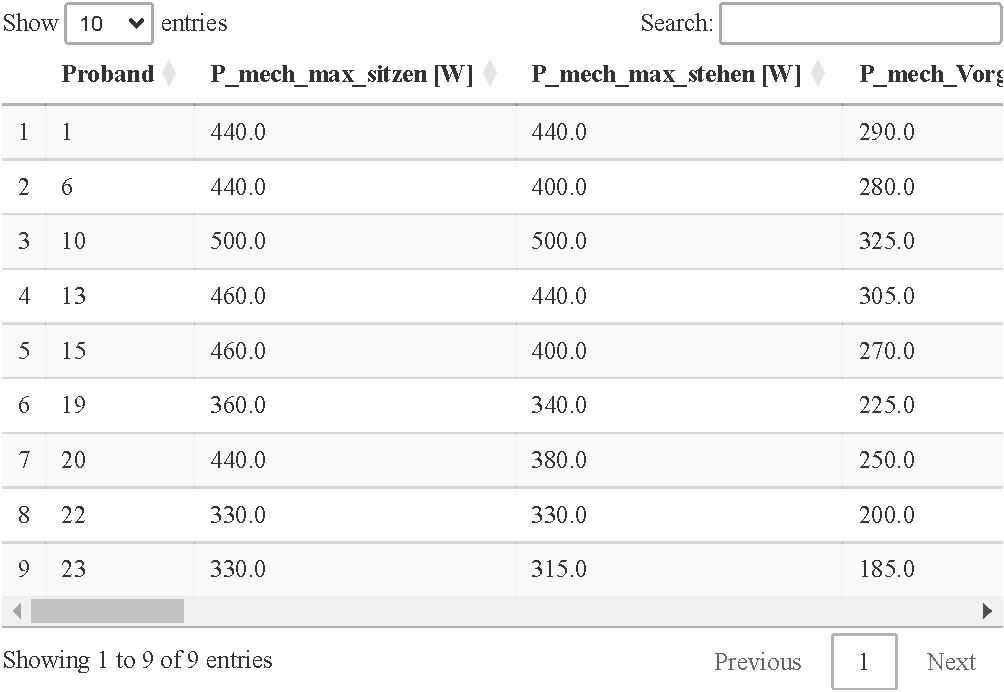
\includegraphics{Drehzahl_Stufentests_files/figure-pdf/tbl-ST_table-1.pdf}

}

\end{table}%

\end{tcolorbox}

\section{Physiologische Parameter beider
Stufentests}\label{physiologische-parameter-beider-stufentests}

Die folgenden Abbildungen zeigen die individuellen Verläufe der
Herzrate, der respiratorischen Parameter \(\dot{V}O_{2}\) und
\(\dot{V}CO_{2}\) sowie der mechanischen Leistung P\textsubscript{mech}
über die Zeit für die Stufentests im Sitzen und Stehen.

\subsection{Proband 01}

\begin{figure}

\centering{

\includegraphics[width=11.45833in,height=4.6875in]{images/p_Stufentest_1_ST1.html}

}

\caption{\label{fig-ST1_1}Belastungsparameter während des Stufentests im
Sitzen: Proband 01}

\end{figure}%

\begin{figure}

\centering{

\includegraphics[width=11.45833in,height=4.6875in]{images/p_Stufentest_1_ST2.html}

}

\caption{\label{fig-ST2_1}Belastungsparameter während des Stufentests im
Stehen: Proband 01}

\end{figure}%

\subsection{Proband 06}

\begin{figure}

\centering{

\includegraphics[width=11.45833in,height=4.6875in]{images/p_Stufentest_6_ST1.html}

}

\caption{\label{fig-ST1_6}Belastungsparameter während des Stufentests im
Sitzen: Proband 06}

\end{figure}%

\begin{figure}

\centering{

\includegraphics[width=11.45833in,height=4.6875in]{images/p_Stufentest_6_ST2.html}

}

\caption{\label{fig-ST2_6}Belastungsparameter während des Stufentests im
Stehen: Proband 06}

\end{figure}%

\subsection{Proband 10}

\begin{figure}

\centering{

\includegraphics[width=11.45833in,height=4.6875in]{images/p_Stufentest_10_ST1.html}

}

\caption{\label{fig-ST1_10}Belastungsparameter während des Stufentests
im Sitzen: Proband 10}

\end{figure}%

\begin{figure}

\centering{

\includegraphics[width=11.45833in,height=4.6875in]{images/p_Stufentest_10_ST2.html}

}

\caption{\label{fig-ST2_10}Belastungsparameter während des Stufentests
im Stehen: Proband 10}

\end{figure}%

\subsection{Proband 13}

\begin{figure}

\centering{

\includegraphics[width=11.45833in,height=4.6875in]{images/p_Stufentest_13_ST1.html}

}

\caption{\label{fig-ST1_13}Belastungsparameter während des Stufentests
im Sitzen: Proband 13}

\end{figure}%

\begin{figure}

\centering{

\includegraphics[width=11.45833in,height=4.6875in]{images/p_Stufentest_13_ST2.html}

}

\caption{\label{fig-ST2_13}Belastungsparameter während des Stufentests
im Stehen: Proband 13}

\end{figure}%

\subsection{Proband 15}

\begin{figure}

\centering{

\includegraphics[width=11.45833in,height=4.6875in]{images/p_Stufentest_15_ST1.html}

}

\caption{\label{fig-ST1_15}Belastungsparameter während des Stufentests
im Sitzen: Proband 15}

\end{figure}%

\begin{figure}

\centering{

\includegraphics[width=11.45833in,height=4.6875in]{images/p_Stufentest_15_ST2.html}

}

\caption{\label{fig-ST2_15}Belastungsparameter während des Stufentests
im Stehen: Proband 15}

\end{figure}%

\subsection{Proband 19}

\begin{figure}

\centering{

\includegraphics[width=11.45833in,height=4.6875in]{images/p_Stufentest_19_ST1.html}

}

\caption{\label{fig-ST1_19}Belastungsparameter während des Stufentests
im Sitzen: Proband 19}

\end{figure}%

\begin{figure}

\centering{

\includegraphics[width=11.45833in,height=4.6875in]{images/p_Stufentest_19_ST2.html}

}

\caption{\label{fig-ST2_19}Belastungsparameter während des Stufentests
im Stehen: Proband 19}

\end{figure}%

\subsection{Proband 20}

\begin{figure}

\centering{

\includegraphics[width=11.45833in,height=4.6875in]{images/p_Stufentest_20_ST1.html}

}

\caption{\label{fig-ST1_20}Belastungsparameter während des Stufentests
im Sitzen: Proband 20}

\end{figure}%

\begin{figure}

\centering{

\includegraphics[width=11.45833in,height=4.6875in]{images/p_Stufentest_20_ST2.html}

}

\caption{\label{fig-ST2_20}Belastungsparameter während des Stufentests
im Stehen: Proband 20}

\end{figure}%

\subsection{Proband 22}

\begin{figure}

\centering{

\includegraphics[width=11.45833in,height=4.6875in]{images/p_Stufentest_22_ST1.html}

}

\caption{\label{fig-ST1_22}Belastungsparameter während des Stufentests
im Sitzen: Proband 22}

\end{figure}%

\begin{figure}

\centering{

\includegraphics[width=11.45833in,height=4.6875in]{images/p_Stufentest_22_ST2.html}

}

\caption{\label{fig-ST2_22}Belastungsparameter während des Stufentests
im Stehen: Proband 22}

\end{figure}%

\subsection{Proband 23}

\begin{figure}

\centering{

\includegraphics[width=11.45833in,height=4.6875in]{images/p_Stufentest_23_ST1.html}

}

\caption{\label{fig-ST1_23}Belastungsparameter während des Stufentests
im Sitzen: Proband 23}

\end{figure}%

\begin{figure}

\centering{

\includegraphics[width=11.45833in,height=4.6875in]{images/p_Stufentest_23_ST2.html}

}

\caption{\label{fig-ST2_23}Belastungsparameter während des Stufentests
im Stehen: Proband 23}

\end{figure}%

\section{Drehzahltest}\label{drehzahltest}

Die folgende Tabelle bietet eine detaillierte deskriptive Auswertung
ausgewählter physiologischer und ergometrischer Parameter des
Drehzahltests, wobei alle Werte als Mittelwert ± Standardabweichung
angegeben werden. Die Daten werden in einer Gesamtübersicht mit
Mittelwerten sowie minimalen und maximalen Messwerten
(Tabelle~\ref{tbl-DT_mean}) dargestellt. Die analysierten Parameter
umfassen die maximale Drehzahl (nD\textsubscript{DT,max}) und die
durchschnittliche Drehzahl der letzten 60 Sekunden
(nD\textsubscript{DT,60}), die berechnete innere Leistung mit Hilfe
biomechanischen Modells sowohl maximal
(P\textsubscript{Int,Modell,DT,max}) als auch gemittelt über die letzten
60 Sekunden (P\textsubscript{Int,Modell,DT,60}), sowie die prozentuale
Ausbelastung des Sauerstoffvolumenstroms im Vergleich zum Stufentest
(\(\dot{V}\text{O}_{2,\text{DT,percent}}\)). Zusätzlich werden die
maximalen Herzraten beider Tests (HR\textsubscript{DT,max},
HR\textsubscript{ST,max}), der durchschnittliche Netto-Wirkungsgrad
(η\textsubscript{DT,netto}), der O\textsubscript{2}-Umsatz pro Watt
(O\textsubscript{2}-Cost of Work\textsubscript{DT,Modell}) und die
O\textsubscript{2}-Kosten der Leerbewegung
(O\textsubscript{2}-Cost\textsubscript{nD,Vorgabe}) dargestellt.

\global\setlength{\Oldarrayrulewidth}{\arrayrulewidth}

\global\setlength{\Oldtabcolsep}{\tabcolsep}

\setlength{\tabcolsep}{2pt}

\renewcommand*{\arraystretch}{1.5}



\providecommand{\ascline}[3]{\noalign{\global\arrayrulewidth #1}\arrayrulecolor[HTML]{#2}\cline{#3}}

\begin{longtable}[c]{cccc}

\caption{\label{tbl-DT_mean}Gemittelte Parameter des Drehzahltests: MW ±
SD, Min \& Max}

\tabularnewline

\hhline{>{\arrayrulecolor[HTML]{A9A9A9}\global\arrayrulewidth=0.5pt}->{\arrayrulecolor[HTML]{A9A9A9}\global\arrayrulewidth=0.5pt}->{\arrayrulecolor[HTML]{A9A9A9}\global\arrayrulewidth=0.5pt}->{\arrayrulecolor[HTML]{A9A9A9}\global\arrayrulewidth=0.5pt}-}

\multicolumn{1}{!{\color[HTML]{A9A9A9}\vrule width 0.5pt}>{\cellcolor[HTML]{EBEBEB}}l}{\textcolor[HTML]{000000}{\fontsize{13}{13}\selectfont{\global\setmainfont{Source Sans Pro}{\textbf{Parameter}}}}} & \multicolumn{1}{!{\color[HTML]{A9A9A9}\vrule width 0.5pt}>{\cellcolor[HTML]{EBEBEB}}c}{\textcolor[HTML]{000000}{\fontsize{13}{13}\selectfont{\global\setmainfont{Source Sans Pro}{\textbf{Mittelwert\ ±\ SD}}}}} & \multicolumn{1}{!{\color[HTML]{A9A9A9}\vrule width 0.5pt}>{\cellcolor[HTML]{EBEBEB}}c}{\textcolor[HTML]{000000}{\fontsize{13}{13}\selectfont{\global\setmainfont{Source Sans Pro}{\textbf{Min}}}}} & \multicolumn{1}{!{\color[HTML]{A9A9A9}\vrule width 0.5pt}>{\cellcolor[HTML]{EBEBEB}}c!{\color[HTML]{A9A9A9}\vrule width 0.5pt}}{\textcolor[HTML]{000000}{\fontsize{13}{13}\selectfont{\global\setmainfont{Source Sans Pro}{\textbf{Max}}}}} \\

\noalign{\global\arrayrulewidth 0.5pt}\arrayrulecolor[HTML]{A9A9A9}

\hhline{|>{\arrayrulecolor[HTML]{A9A9A9}\global\arrayrulewidth=0.5pt}-|>{\arrayrulecolor[HTML]{A9A9A9}\global\arrayrulewidth=0.5pt}-|>{\arrayrulecolor[HTML]{A9A9A9}\global\arrayrulewidth=0.5pt}-|>{\arrayrulecolor[HTML]{A9A9A9}\global\arrayrulewidth=0.5pt}-}\endfirsthead 

\hhline{>{\arrayrulecolor[HTML]{A9A9A9}\global\arrayrulewidth=0.5pt}->{\arrayrulecolor[HTML]{A9A9A9}\global\arrayrulewidth=0.5pt}->{\arrayrulecolor[HTML]{A9A9A9}\global\arrayrulewidth=0.5pt}->{\arrayrulecolor[HTML]{A9A9A9}\global\arrayrulewidth=0.5pt}-}

\multicolumn{1}{!{\color[HTML]{A9A9A9}\vrule width 0.5pt}>{\cellcolor[HTML]{EBEBEB}}l}{\textcolor[HTML]{000000}{\fontsize{13}{13}\selectfont{\global\setmainfont{Source Sans Pro}{\textbf{Parameter}}}}} & \multicolumn{1}{!{\color[HTML]{A9A9A9}\vrule width 0.5pt}>{\cellcolor[HTML]{EBEBEB}}c}{\textcolor[HTML]{000000}{\fontsize{13}{13}\selectfont{\global\setmainfont{Source Sans Pro}{\textbf{Mittelwert\ ±\ SD}}}}} & \multicolumn{1}{!{\color[HTML]{A9A9A9}\vrule width 0.5pt}>{\cellcolor[HTML]{EBEBEB}}c}{\textcolor[HTML]{000000}{\fontsize{13}{13}\selectfont{\global\setmainfont{Source Sans Pro}{\textbf{Min}}}}} & \multicolumn{1}{!{\color[HTML]{A9A9A9}\vrule width 0.5pt}>{\cellcolor[HTML]{EBEBEB}}c!{\color[HTML]{A9A9A9}\vrule width 0.5pt}}{\textcolor[HTML]{000000}{\fontsize{13}{13}\selectfont{\global\setmainfont{Source Sans Pro}{\textbf{Max}}}}} \\

\noalign{\global\arrayrulewidth 0.5pt}\arrayrulecolor[HTML]{A9A9A9}

\hhline{|>{\arrayrulecolor[HTML]{A9A9A9}\global\arrayrulewidth=0.5pt}-|>{\arrayrulecolor[HTML]{A9A9A9}\global\arrayrulewidth=0.5pt}-|>{\arrayrulecolor[HTML]{A9A9A9}\global\arrayrulewidth=0.5pt}-|>{\arrayrulecolor[HTML]{A9A9A9}\global\arrayrulewidth=0.5pt}-}\endhead



\multicolumn{1}{!{\color[HTML]{A9A9A9}\vrule width 0.5pt}>{\cellcolor[HTML]{F9F9F9}}l}{\textcolor[HTML]{000000}{\fontsize{13}{13}\selectfont{\global\setmainfont{Source Sans Pro}{nD}}}\textcolor[HTML]{000000}{\fontsize{13}{13}\selectfont{\global\setmainfont{Source Sans Pro}{\textsubscript{DT,max}}}}\textcolor[HTML]{000000}{\fontsize{13}{13}\selectfont{\global\setmainfont{Source Sans Pro}{\ [min⁻¹]}}}} & \multicolumn{1}{!{\color[HTML]{A9A9A9}\vrule width 0.5pt}>{\cellcolor[HTML]{F9F9F9}}c}{\textcolor[HTML]{000000}{\fontsize{13}{13}\selectfont{\global\setmainfont{Source Sans Pro}{173.7\ ±\ 6.5}}}} & \multicolumn{1}{!{\color[HTML]{A9A9A9}\vrule width 0.5pt}>{\cellcolor[HTML]{F9F9F9}}c}{\textcolor[HTML]{000000}{\fontsize{13}{13}\selectfont{\global\setmainfont{Source Sans Pro}{162.5}}}} & \multicolumn{1}{!{\color[HTML]{A9A9A9}\vrule width 0.5pt}>{\cellcolor[HTML]{F9F9F9}}c!{\color[HTML]{A9A9A9}\vrule width 0.5pt}}{\textcolor[HTML]{000000}{\fontsize{13}{13}\selectfont{\global\setmainfont{Source Sans Pro}{183.0}}}} \\

\noalign{\global\arrayrulewidth 0.5pt}\arrayrulecolor[HTML]{A9A9A9}

\hhline{|>{\arrayrulecolor[HTML]{D3D3D3}\global\arrayrulewidth=0.5pt}-|>{\arrayrulecolor[HTML]{D3D3D3}\global\arrayrulewidth=0.5pt}-|>{\arrayrulecolor[HTML]{D3D3D3}\global\arrayrulewidth=0.5pt}-|>{\arrayrulecolor[HTML]{D3D3D3}\global\arrayrulewidth=0.5pt}-}



\multicolumn{1}{!{\color[HTML]{A9A9A9}\vrule width 0.5pt}>{\cellcolor[HTML]{FFFFFF}}l}{\textcolor[HTML]{000000}{\fontsize{13}{13}\selectfont{\global\setmainfont{Source Sans Pro}{nD}}}\textcolor[HTML]{000000}{\fontsize{13}{13}\selectfont{\global\setmainfont{Source Sans Pro}{\textsubscript{DT,60}}}}\textcolor[HTML]{000000}{\fontsize{13}{13}\selectfont{\global\setmainfont{Source Sans Pro}{\ [min⁻¹]}}}} & \multicolumn{1}{!{\color[HTML]{A9A9A9}\vrule width 0.5pt}>{\cellcolor[HTML]{FFFFFF}}c}{\textcolor[HTML]{000000}{\fontsize{13}{13}\selectfont{\global\setmainfont{Source Sans Pro}{168.7\ ±\ 6.4}}}} & \multicolumn{1}{!{\color[HTML]{A9A9A9}\vrule width 0.5pt}>{\cellcolor[HTML]{FFFFFF}}c}{\textcolor[HTML]{000000}{\fontsize{13}{13}\selectfont{\global\setmainfont{Source Sans Pro}{159.2}}}} & \multicolumn{1}{!{\color[HTML]{A9A9A9}\vrule width 0.5pt}>{\cellcolor[HTML]{FFFFFF}}c!{\color[HTML]{A9A9A9}\vrule width 0.5pt}}{\textcolor[HTML]{000000}{\fontsize{13}{13}\selectfont{\global\setmainfont{Source Sans Pro}{177.6}}}} \\

\noalign{\global\arrayrulewidth 0.5pt}\arrayrulecolor[HTML]{A9A9A9}

\hhline{|>{\arrayrulecolor[HTML]{D3D3D3}\global\arrayrulewidth=0.5pt}-|>{\arrayrulecolor[HTML]{D3D3D3}\global\arrayrulewidth=0.5pt}-|>{\arrayrulecolor[HTML]{D3D3D3}\global\arrayrulewidth=0.5pt}-|>{\arrayrulecolor[HTML]{D3D3D3}\global\arrayrulewidth=0.5pt}-}



\multicolumn{1}{!{\color[HTML]{A9A9A9}\vrule width 0.5pt}>{\cellcolor[HTML]{F9F9F9}}l}{\textcolor[HTML]{000000}{\fontsize{13}{13}\selectfont{\global\setmainfont{Source Sans Pro}{P}}}\textcolor[HTML]{000000}{\fontsize{13}{13}\selectfont{\global\setmainfont{Source Sans Pro}{\textsubscript{Int,Modell,DT,max}}}}\textcolor[HTML]{000000}{\fontsize{13}{13}\selectfont{\global\setmainfont{Source Sans Pro}{\ [W]}}}} & \multicolumn{1}{!{\color[HTML]{A9A9A9}\vrule width 0.5pt}>{\cellcolor[HTML]{F9F9F9}}c}{\textcolor[HTML]{000000}{\fontsize{13}{13}\selectfont{\global\setmainfont{Source Sans Pro}{269.1\ ±\ 48.6}}}} & \multicolumn{1}{!{\color[HTML]{A9A9A9}\vrule width 0.5pt}>{\cellcolor[HTML]{F9F9F9}}c}{\textcolor[HTML]{000000}{\fontsize{13}{13}\selectfont{\global\setmainfont{Source Sans Pro}{192.8}}}} & \multicolumn{1}{!{\color[HTML]{A9A9A9}\vrule width 0.5pt}>{\cellcolor[HTML]{F9F9F9}}c!{\color[HTML]{A9A9A9}\vrule width 0.5pt}}{\textcolor[HTML]{000000}{\fontsize{13}{13}\selectfont{\global\setmainfont{Source Sans Pro}{337.5}}}} \\

\noalign{\global\arrayrulewidth 0.5pt}\arrayrulecolor[HTML]{A9A9A9}

\hhline{|>{\arrayrulecolor[HTML]{D3D3D3}\global\arrayrulewidth=0.5pt}-|>{\arrayrulecolor[HTML]{D3D3D3}\global\arrayrulewidth=0.5pt}-|>{\arrayrulecolor[HTML]{D3D3D3}\global\arrayrulewidth=0.5pt}-|>{\arrayrulecolor[HTML]{D3D3D3}\global\arrayrulewidth=0.5pt}-}



\multicolumn{1}{!{\color[HTML]{A9A9A9}\vrule width 0.5pt}>{\cellcolor[HTML]{FFFFFF}}l}{\textcolor[HTML]{000000}{\fontsize{13}{13}\selectfont{\global\setmainfont{Source Sans Pro}{P}}}\textcolor[HTML]{000000}{\fontsize{13}{13}\selectfont{\global\setmainfont{Source Sans Pro}{\textsubscript{Int,Modell,DT,60}}}}\textcolor[HTML]{000000}{\fontsize{13}{13}\selectfont{\global\setmainfont{Source Sans Pro}{\ [W]}}}} & \multicolumn{1}{!{\color[HTML]{A9A9A9}\vrule width 0.5pt}>{\cellcolor[HTML]{FFFFFF}}c}{\textcolor[HTML]{000000}{\fontsize{13}{13}\selectfont{\global\setmainfont{Source Sans Pro}{251.4\ ±\ 42.9}}}} & \multicolumn{1}{!{\color[HTML]{A9A9A9}\vrule width 0.5pt}>{\cellcolor[HTML]{FFFFFF}}c}{\textcolor[HTML]{000000}{\fontsize{13}{13}\selectfont{\global\setmainfont{Source Sans Pro}{188.4}}}} & \multicolumn{1}{!{\color[HTML]{A9A9A9}\vrule width 0.5pt}>{\cellcolor[HTML]{FFFFFF}}c!{\color[HTML]{A9A9A9}\vrule width 0.5pt}}{\textcolor[HTML]{000000}{\fontsize{13}{13}\selectfont{\global\setmainfont{Source Sans Pro}{323.8}}}} \\

\noalign{\global\arrayrulewidth 0.5pt}\arrayrulecolor[HTML]{A9A9A9}

\hhline{|>{\arrayrulecolor[HTML]{D3D3D3}\global\arrayrulewidth=0.5pt}-|>{\arrayrulecolor[HTML]{D3D3D3}\global\arrayrulewidth=0.5pt}-|>{\arrayrulecolor[HTML]{D3D3D3}\global\arrayrulewidth=0.5pt}-|>{\arrayrulecolor[HTML]{D3D3D3}\global\arrayrulewidth=0.5pt}-}



\multicolumn{1}{!{\color[HTML]{A9A9A9}\vrule width 0.5pt}>{\cellcolor[HTML]{F9F9F9}}l}{\textcolor[HTML]{000000}{\fontsize{13}{13}\selectfont{\global\setmainfont{Source Sans Pro}{V̇O}}}\textcolor[HTML]{000000}{\fontsize{13}{13}\selectfont{\global\setmainfont{Source Sans Pro}{\textsubscript{2,DT,percent}}}}\textcolor[HTML]{000000}{\fontsize{13}{13}\selectfont{\global\setmainfont{Source Sans Pro}{\ [\%]}}}} & \multicolumn{1}{!{\color[HTML]{A9A9A9}\vrule width 0.5pt}>{\cellcolor[HTML]{F9F9F9}}c}{\textcolor[HTML]{000000}{\fontsize{13}{13}\selectfont{\global\setmainfont{Source Sans Pro}{93.9\ ±\ 3.6}}}} & \multicolumn{1}{!{\color[HTML]{A9A9A9}\vrule width 0.5pt}>{\cellcolor[HTML]{F9F9F9}}c}{\textcolor[HTML]{000000}{\fontsize{13}{13}\selectfont{\global\setmainfont{Source Sans Pro}{88.0}}}} & \multicolumn{1}{!{\color[HTML]{A9A9A9}\vrule width 0.5pt}>{\cellcolor[HTML]{F9F9F9}}c!{\color[HTML]{A9A9A9}\vrule width 0.5pt}}{\textcolor[HTML]{000000}{\fontsize{13}{13}\selectfont{\global\setmainfont{Source Sans Pro}{97.2}}}} \\

\noalign{\global\arrayrulewidth 0.5pt}\arrayrulecolor[HTML]{A9A9A9}

\hhline{|>{\arrayrulecolor[HTML]{D3D3D3}\global\arrayrulewidth=0.5pt}-|>{\arrayrulecolor[HTML]{D3D3D3}\global\arrayrulewidth=0.5pt}-|>{\arrayrulecolor[HTML]{D3D3D3}\global\arrayrulewidth=0.5pt}-|>{\arrayrulecolor[HTML]{D3D3D3}\global\arrayrulewidth=0.5pt}-}



\multicolumn{1}{!{\color[HTML]{A9A9A9}\vrule width 0.5pt}>{\cellcolor[HTML]{FFFFFF}}l}{\textcolor[HTML]{000000}{\fontsize{13}{13}\selectfont{\global\setmainfont{Source Sans Pro}{HR}}}\textcolor[HTML]{000000}{\fontsize{13}{13}\selectfont{\global\setmainfont{Source Sans Pro}{\textsubscript{DT,max}}}}\textcolor[HTML]{000000}{\fontsize{13}{13}\selectfont{\global\setmainfont{Source Sans Pro}{\ [min⁻¹]}}}} & \multicolumn{1}{!{\color[HTML]{A9A9A9}\vrule width 0.5pt}>{\cellcolor[HTML]{FFFFFF}}c}{\textcolor[HTML]{000000}{\fontsize{13}{13}\selectfont{\global\setmainfont{Source Sans Pro}{181.5\ ±\ 5.6}}}} & \multicolumn{1}{!{\color[HTML]{A9A9A9}\vrule width 0.5pt}>{\cellcolor[HTML]{FFFFFF}}c}{\textcolor[HTML]{000000}{\fontsize{13}{13}\selectfont{\global\setmainfont{Source Sans Pro}{174.0}}}} & \multicolumn{1}{!{\color[HTML]{A9A9A9}\vrule width 0.5pt}>{\cellcolor[HTML]{FFFFFF}}c!{\color[HTML]{A9A9A9}\vrule width 0.5pt}}{\textcolor[HTML]{000000}{\fontsize{13}{13}\selectfont{\global\setmainfont{Source Sans Pro}{191.0}}}} \\

\noalign{\global\arrayrulewidth 0.5pt}\arrayrulecolor[HTML]{A9A9A9}

\hhline{|>{\arrayrulecolor[HTML]{D3D3D3}\global\arrayrulewidth=0.5pt}-|>{\arrayrulecolor[HTML]{D3D3D3}\global\arrayrulewidth=0.5pt}-|>{\arrayrulecolor[HTML]{D3D3D3}\global\arrayrulewidth=0.5pt}-|>{\arrayrulecolor[HTML]{D3D3D3}\global\arrayrulewidth=0.5pt}-}



\multicolumn{1}{!{\color[HTML]{A9A9A9}\vrule width 0.5pt}>{\cellcolor[HTML]{F9F9F9}}l}{\textcolor[HTML]{000000}{\fontsize{13}{13}\selectfont{\global\setmainfont{Source Sans Pro}{HR}}}\textcolor[HTML]{000000}{\fontsize{13}{13}\selectfont{\global\setmainfont{Source Sans Pro}{\textsubscript{ST,max}}}}\textcolor[HTML]{000000}{\fontsize{13}{13}\selectfont{\global\setmainfont{Source Sans Pro}{\ [min⁻¹]}}}} & \multicolumn{1}{!{\color[HTML]{A9A9A9}\vrule width 0.5pt}>{\cellcolor[HTML]{F9F9F9}}c}{\textcolor[HTML]{000000}{\fontsize{13}{13}\selectfont{\global\setmainfont{Source Sans Pro}{178.7\ ±\ 7.5}}}} & \multicolumn{1}{!{\color[HTML]{A9A9A9}\vrule width 0.5pt}>{\cellcolor[HTML]{F9F9F9}}c}{\textcolor[HTML]{000000}{\fontsize{13}{13}\selectfont{\global\setmainfont{Source Sans Pro}{169.0}}}} & \multicolumn{1}{!{\color[HTML]{A9A9A9}\vrule width 0.5pt}>{\cellcolor[HTML]{F9F9F9}}c!{\color[HTML]{A9A9A9}\vrule width 0.5pt}}{\textcolor[HTML]{000000}{\fontsize{13}{13}\selectfont{\global\setmainfont{Source Sans Pro}{192.0}}}} \\

\noalign{\global\arrayrulewidth 0.5pt}\arrayrulecolor[HTML]{A9A9A9}

\hhline{|>{\arrayrulecolor[HTML]{D3D3D3}\global\arrayrulewidth=0.5pt}-|>{\arrayrulecolor[HTML]{D3D3D3}\global\arrayrulewidth=0.5pt}-|>{\arrayrulecolor[HTML]{D3D3D3}\global\arrayrulewidth=0.5pt}-|>{\arrayrulecolor[HTML]{D3D3D3}\global\arrayrulewidth=0.5pt}-}



\multicolumn{1}{!{\color[HTML]{A9A9A9}\vrule width 0.5pt}>{\cellcolor[HTML]{FFFFFF}}l}{\textcolor[HTML]{000000}{\fontsize{13}{13}\selectfont{\global\setmainfont{Source Sans Pro}{η}}}\textcolor[HTML]{000000}{\fontsize{13}{13}\selectfont{\global\setmainfont{Source Sans Pro}{\textsubscript{DT,netto}}}}\textcolor[HTML]{000000}{\fontsize{13}{13}\selectfont{\global\setmainfont{Source Sans Pro}{\ [\%]}}}} & \multicolumn{1}{!{\color[HTML]{A9A9A9}\vrule width 0.5pt}>{\cellcolor[HTML]{FFFFFF}}c}{\textcolor[HTML]{000000}{\fontsize{13}{13}\selectfont{\global\setmainfont{Source Sans Pro}{18.49\ ±\ 2.13}}}} & \multicolumn{1}{!{\color[HTML]{A9A9A9}\vrule width 0.5pt}>{\cellcolor[HTML]{FFFFFF}}c}{\textcolor[HTML]{000000}{\fontsize{13}{13}\selectfont{\global\setmainfont{Source Sans Pro}{16.40}}}} & \multicolumn{1}{!{\color[HTML]{A9A9A9}\vrule width 0.5pt}>{\cellcolor[HTML]{FFFFFF}}c!{\color[HTML]{A9A9A9}\vrule width 0.5pt}}{\textcolor[HTML]{000000}{\fontsize{13}{13}\selectfont{\global\setmainfont{Source Sans Pro}{23.10}}}} \\

\noalign{\global\arrayrulewidth 0.5pt}\arrayrulecolor[HTML]{A9A9A9}

\hhline{|>{\arrayrulecolor[HTML]{D3D3D3}\global\arrayrulewidth=0.5pt}-|>{\arrayrulecolor[HTML]{D3D3D3}\global\arrayrulewidth=0.5pt}-|>{\arrayrulecolor[HTML]{D3D3D3}\global\arrayrulewidth=0.5pt}-|>{\arrayrulecolor[HTML]{D3D3D3}\global\arrayrulewidth=0.5pt}-}



\multicolumn{1}{!{\color[HTML]{A9A9A9}\vrule width 0.5pt}>{\cellcolor[HTML]{F9F9F9}}l}{\textcolor[HTML]{000000}{\fontsize{13}{13}\selectfont{\global\setmainfont{Source Sans Pro}{O}}}\textcolor[HTML]{000000}{\fontsize{13}{13}\selectfont{\global\setmainfont{Source Sans Pro}{\textsubscript{2}}}}\textcolor[HTML]{000000}{\fontsize{13}{13}\selectfont{\global\setmainfont{Source Sans Pro}{-Cost\ of\ Work}}}\textcolor[HTML]{000000}{\fontsize{13}{13}\selectfont{\global\setmainfont{Source Sans Pro}{\textsubscript{DT,Modell}}}}\textcolor[HTML]{000000}{\fontsize{13}{13}\selectfont{\global\setmainfont{Source Sans Pro}{\ [ml·min⁻¹·W⁻¹]}}}} & \multicolumn{1}{!{\color[HTML]{A9A9A9}\vrule width 0.5pt}>{\cellcolor[HTML]{F9F9F9}}c}{\textcolor[HTML]{000000}{\fontsize{13}{13}\selectfont{\global\setmainfont{Source Sans Pro}{14.867}}}} & \multicolumn{1}{!{\color[HTML]{A9A9A9}\vrule width 0.5pt}>{\cellcolor[HTML]{F9F9F9}}c}{\textcolor[HTML]{000000}{\fontsize{13}{13}\selectfont{\global\setmainfont{Source Sans Pro}{-}}}} & \multicolumn{1}{!{\color[HTML]{A9A9A9}\vrule width 0.5pt}>{\cellcolor[HTML]{F9F9F9}}c!{\color[HTML]{A9A9A9}\vrule width 0.5pt}}{\textcolor[HTML]{000000}{\fontsize{13}{13}\selectfont{\global\setmainfont{Source Sans Pro}{-}}}} \\

\noalign{\global\arrayrulewidth 0.5pt}\arrayrulecolor[HTML]{A9A9A9}

\hhline{|>{\arrayrulecolor[HTML]{D3D3D3}\global\arrayrulewidth=0.5pt}-|>{\arrayrulecolor[HTML]{D3D3D3}\global\arrayrulewidth=0.5pt}-|>{\arrayrulecolor[HTML]{D3D3D3}\global\arrayrulewidth=0.5pt}-|>{\arrayrulecolor[HTML]{D3D3D3}\global\arrayrulewidth=0.5pt}-}



\multicolumn{1}{!{\color[HTML]{A9A9A9}\vrule width 0.5pt}>{\cellcolor[HTML]{FFFFFF}}l}{\textcolor[HTML]{000000}{\fontsize{13}{13}\selectfont{\global\setmainfont{Source Sans Pro}{O}}}\textcolor[HTML]{000000}{\fontsize{13}{13}\selectfont{\global\setmainfont{Source Sans Pro}{\textsubscript{2}}}}\textcolor[HTML]{000000}{\fontsize{13}{13}\selectfont{\global\setmainfont{Source Sans Pro}{-Cost}}}\textcolor[HTML]{000000}{\fontsize{13}{13}\selectfont{\global\setmainfont{Source Sans Pro}{\textsubscript{nD,Vorgabe}}}}\textcolor[HTML]{000000}{\fontsize{13}{13}\selectfont{\global\setmainfont{Source Sans Pro}{\ [l·min⁻¹]}}}} & \multicolumn{1}{!{\color[HTML]{A9A9A9}\vrule width 0.5pt}>{\cellcolor[HTML]{FFFFFF}}c}{\textcolor[HTML]{000000}{\fontsize{13}{13}\selectfont{\global\setmainfont{Source Sans Pro}{0.556\ ±\ 0.165}}}} & \multicolumn{1}{!{\color[HTML]{A9A9A9}\vrule width 0.5pt}>{\cellcolor[HTML]{FFFFFF}}c}{\textcolor[HTML]{000000}{\fontsize{13}{13}\selectfont{\global\setmainfont{Source Sans Pro}{0.329}}}} & \multicolumn{1}{!{\color[HTML]{A9A9A9}\vrule width 0.5pt}>{\cellcolor[HTML]{FFFFFF}}c!{\color[HTML]{A9A9A9}\vrule width 0.5pt}}{\textcolor[HTML]{000000}{\fontsize{13}{13}\selectfont{\global\setmainfont{Source Sans Pro}{0.805}}}} \\

\noalign{\global\arrayrulewidth 0.5pt}\arrayrulecolor[HTML]{A9A9A9}

\hhline{|>{\arrayrulecolor[HTML]{D3D3D3}\global\arrayrulewidth=0.5pt}-|>{\arrayrulecolor[HTML]{D3D3D3}\global\arrayrulewidth=0.5pt}-|>{\arrayrulecolor[HTML]{D3D3D3}\global\arrayrulewidth=0.5pt}-|>{\arrayrulecolor[HTML]{D3D3D3}\global\arrayrulewidth=0.5pt}-}



\multicolumn{4}{!{\color[HTML]{A9A9A9}\vrule width 0.5pt}>{}l!{\color[HTML]{A9A9A9}\vrule width 0.5pt}}{\textcolor[HTML]{000000}{\fontsize{11}{13}\selectfont{\global\setmainfont{Source Sans Pro}{nD}}}\textcolor[HTML]{000000}{\fontsize{11}{13}\selectfont{\global\setmainfont{Source Sans Pro}{\textsubscript{DT,max}}}}\textcolor[HTML]{000000}{\fontsize{11}{13}\selectfont{\global\setmainfont{Source Sans Pro}{\ [min⁻¹]:\ Maximale\ Drehzahl\ im\ DT;\ }}}\textcolor[HTML]{000000}{\fontsize{11}{13}\selectfont{\global\setmainfont{Source Sans Pro}{nD}}}\textcolor[HTML]{000000}{\fontsize{11}{13}\selectfont{\global\setmainfont{Source Sans Pro}{\textsubscript{DT,60}}}}\textcolor[HTML]{000000}{\fontsize{11}{13}\selectfont{\global\setmainfont{Source Sans Pro}{\ [min⁻¹]:\ Durchschnittliche\ Drehzahl\ in\ den\ letzten\ 60s\ des\ DT;\ }}}\textcolor[HTML]{000000}{\fontsize{11}{13}\selectfont{\global\setmainfont{Source Sans Pro}{P}}}\textcolor[HTML]{000000}{\fontsize{11}{13}\selectfont{\global\setmainfont{Source Sans Pro}{\textsubscript{Int,Modell,DT,max}}}}\textcolor[HTML]{000000}{\fontsize{11}{13}\selectfont{\global\setmainfont{Source Sans Pro}{\ [W]:\ Maximale\ interne\ Leistung\ während\ des\ DT\ basierend\ auf\ biomechanischer\ Modellsimulation;\ }}}\textcolor[HTML]{000000}{\fontsize{11}{13}\selectfont{\global\setmainfont{Source Sans Pro}{P}}}\textcolor[HTML]{000000}{\fontsize{11}{13}\selectfont{\global\setmainfont{Source Sans Pro}{\textsubscript{Int,Modell,DT,60}}}}\textcolor[HTML]{000000}{\fontsize{11}{13}\selectfont{\global\setmainfont{Source Sans Pro}{\ [W]:\ Durchschnittliche\ interne\ Leistung\ der\ letzten\ 60s\ des\ DT;\ }}}\textcolor[HTML]{000000}{\fontsize{11}{13}\selectfont{\global\setmainfont{Source Sans Pro}{V̇O}}}\textcolor[HTML]{000000}{\fontsize{11}{13}\selectfont{\global\setmainfont{Source Sans Pro}{\textsubscript{2,DT,percent}}}}\textcolor[HTML]{000000}{\fontsize{11}{13}\selectfont{\global\setmainfont{Source Sans Pro}{\ [\%]:\ Prozentuale\ Auslastung\ der\ V̇O}}}\textcolor[HTML]{000000}{\fontsize{11}{13}\selectfont{\global\setmainfont{Source Sans Pro}{\textsubscript{2}}}}\textcolor[HTML]{000000}{\fontsize{11}{13}\selectfont{\global\setmainfont{Source Sans Pro}{\ im\ DT\ im\ Vergleich\ zur\ maximalen\ V̇O}}}\textcolor[HTML]{000000}{\fontsize{11}{13}\selectfont{\global\setmainfont{Source Sans Pro}{\textsubscript{2}}}}\textcolor[HTML]{000000}{\fontsize{11}{13}\selectfont{\global\setmainfont{Source Sans Pro}{\ im\ Stufentest;\ }}}\textcolor[HTML]{000000}{\fontsize{11}{13}\selectfont{\global\setmainfont{Source Sans Pro}{HR}}}\textcolor[HTML]{000000}{\fontsize{11}{13}\selectfont{\global\setmainfont{Source Sans Pro}{\textsubscript{DT,max}}}}\textcolor[HTML]{000000}{\fontsize{11}{13}\selectfont{\global\setmainfont{Source Sans Pro}{\ [min⁻¹]:\ Maximale\ Herzrate\ im\ DT;\ }}}\textcolor[HTML]{000000}{\fontsize{11}{13}\selectfont{\global\setmainfont{Source Sans Pro}{HR}}}\textcolor[HTML]{000000}{\fontsize{11}{13}\selectfont{\global\setmainfont{Source Sans Pro}{\textsubscript{ST,max}}}}\textcolor[HTML]{000000}{\fontsize{11}{13}\selectfont{\global\setmainfont{Source Sans Pro}{\ [min⁻¹]:\ Maximale\ Herzrate\ im\ ST;\ }}}\textcolor[HTML]{000000}{\fontsize{11}{13}\selectfont{\global\setmainfont{Source Sans Pro}{η}}}\textcolor[HTML]{000000}{\fontsize{11}{13}\selectfont{\global\setmainfont{Source Sans Pro}{\textsubscript{DT,netto}}}}\textcolor[HTML]{000000}{\fontsize{11}{13}\selectfont{\global\setmainfont{Source Sans Pro}{\ [\%]:\ Netto-Wirkungsgrad\ im\ Drehzahltest\ ab\ nD\ >\ 80;\ }}}\textcolor[HTML]{000000}{\fontsize{11}{13}\selectfont{\global\setmainfont{Source Sans Pro}{O}}}\textcolor[HTML]{000000}{\fontsize{11}{13}\selectfont{\global\setmainfont{Source Sans Pro}{\textsubscript{2}}}}\textcolor[HTML]{000000}{\fontsize{11}{13}\selectfont{\global\setmainfont{Source Sans Pro}{-Cost\ of\ Work}}}\textcolor[HTML]{000000}{\fontsize{11}{13}\selectfont{\global\setmainfont{Source Sans Pro}{\textsubscript{DT,Modell}}}}\textcolor[HTML]{000000}{\fontsize{11}{13}\selectfont{\global\setmainfont{Source Sans Pro}{\ [ml·min⁻¹·W⁻¹]:\ O₂-Umsatz\ pro\ Watt\ P}}}\textcolor[HTML]{000000}{\fontsize{11}{13}\selectfont{\global\setmainfont{Source Sans Pro}{\textsubscript{Int,Modell}}}}\textcolor[HTML]{000000}{\fontsize{11}{13}\selectfont{\global\setmainfont{Source Sans Pro}{\ im\ DT;\ }}}\textcolor[HTML]{000000}{\fontsize{11}{13}\selectfont{\global\setmainfont{Source Sans Pro}{O}}}\textcolor[HTML]{000000}{\fontsize{11}{13}\selectfont{\global\setmainfont{Source Sans Pro}{\textsubscript{2}}}}\textcolor[HTML]{000000}{\fontsize{11}{13}\selectfont{\global\setmainfont{Source Sans Pro}{-Kosten\ Leerbewegung\ n}}}\textcolor[HTML]{000000}{\fontsize{11}{13}\selectfont{\global\setmainfont{Source Sans Pro}{\textsubscript{D,Vorgabe}}}}\textcolor[HTML]{000000}{\fontsize{11}{13}\selectfont{\global\setmainfont{Source Sans Pro}{\ [l·min⁻¹]:\ O₂-Umsatz\ der\ Leerbewegung\ bei\ vorgegebener\ nD\ an\ Testtag\ 2\ für\ die\ Berechnung\ von\ η}}}\textcolor[HTML]{000000}{\fontsize{11}{13}\selectfont{\global\setmainfont{Source Sans Pro}{\textsubscript{Arbeit}}}}} \\

\noalign{\global\arrayrulewidth 0.5pt}\arrayrulecolor[HTML]{A9A9A9}

\hhline{|>{\arrayrulecolor[HTML]{A9A9A9}\global\arrayrulewidth=0.5pt}-|>{\arrayrulecolor[HTML]{A9A9A9}\global\arrayrulewidth=0.5pt}-|>{\arrayrulecolor[HTML]{A9A9A9}\global\arrayrulewidth=0.5pt}-|>{\arrayrulecolor[HTML]{A9A9A9}\global\arrayrulewidth=0.5pt}-}


\end{longtable}

\arrayrulecolor[HTML]{000000}

\global\setlength{\arrayrulewidth}{\Oldarrayrulewidth}

\global\setlength{\tabcolsep}{\Oldtabcolsep}

\renewcommand*{\arraystretch}{1}

\paragraph{Drehzahl}\label{drehzahl}

Die maximale erreichte Drehzahl nD\textsubscript{DT,max} während des
Drehzahltests betrug im Mittel aller Durchgänge der Probanden 173.7 ±
6.5 min\textsuperscript{-1}, wobei die höchste erreichte Drehzahl bei
183.0 min\textsuperscript{-1} und die niedrigste bei 162.5
min\textsuperscript{-1} lag. Im Mittel aller Probanden lag die Drehzahl
während der letzten 60 Sekunden nD\textsubscript{DT,60} bei 168.7 ± 6.4
min\textsuperscript{-1} (R: 159.2-177.6 min\textsuperscript{-1}).

\paragraph{Innere Leistung}\label{innere-leistung}

Die mittels biomechanischer Modellsimulation berechnete maximale innere
Leistung P\textsubscript{Int,Modell,DT,max} während des Drehzahltests
lag zwischen 192.8 und 337.5 W und betrug im Mittel aller Probanden
269.1 ± 48.6 W. Die durchschnittliche P\textsubscript{Int,Modell,DT,max}
in den letzten 60 Sekunden P\textsubscript{Int,Modell,DT,60} lag bei
251.4 ± 42.9 W (R: 188.4-323.8 W).

\paragraph{Ventilatorische und physiologische
Kenngrößen}\label{ventilatorische-und-physiologische-kenngruxf6uxdfen}

Die prozentuale Auslastung des Sauerstoffvolumenstroms
\(\dot{V}O_{2,DT,percent}\) im Vergleich zum maximalen gemessenen
Sauerstoffvolumenstrom während der Stufentests erreichte im Mittel 93.9
± 3.6\% und blieb auch im Maximum mit 97.2\% unter dem maximalen
Sauerstoffvolumenstrom der Stufentests. Die maximale Herzrate im
Drehzahltest HR\textsubscript{DT,max} lag durchschnittlich bei 181.5 ±
5.6 min\textsuperscript{-1} (Range (R): 174-191 min\textsuperscript{-1})
und damit im Mittel höher als die maximale Herzrate der Stufentests
HR\textsubscript{ST,max} von 178.7 ± 7.5 min\textsuperscript{-1} (R:
169-192 min\textsuperscript{-1}).

\paragraph{Netto-Wirkungsgrad}\label{netto-wirkungsgrad}

Der Netto-Wirkungsgrad η\textsubscript{DT,netto}, der mit der
P\textsubscript{Int,Modell,DT} kalkuliert wurde, betrug während des
Drehzahltests für die Drehzahlwerte über 80 min\textsuperscript{-1} im
Durchschnitt 18.49 ± 2.13\%, mit einem Maximum von 23.10\% und einem
Minimum von 16.40\%.

\paragraph{\texorpdfstring{Zusammenhang des VO\textsubscript{2,net} und
P\textsubscript{Int,Modell,DT}}{Zusammenhang des VO2,net und PInt,Modell,DT}}\label{zusammenhang-des-vo2net-und-pintmodelldt}

Der Sauerstoffumsatz pro Watt P\textsubscript{Int,Modell,DT}
(O\textsubscript{2}-Cost of Work\textsubscript{DT,Modell}) lag bei
14.867 ml·min\textsuperscript{-1}·W\textsuperscript{-1} und damit über
den in der Literatur beschriebenen Werten von 8.5-12.0
ml·min\textsuperscript{-1}·W\textsuperscript{-1} für die
Fahrradergometrie (Heck et al., 2022; Özyener et al., 2001; Rassouli \&
Thurnheer, 2015; Wasserman et al., 2011) (siehe
Abbildung~\ref{fig-DT_O2cost_all} \&
Abbildung~\ref{fig-DT_O2cost_mean}).

\subsection{Alle Probanden}

\begin{figure}

\centering{

\includegraphics[width=11.45833in,height=4.6875in]{images/p_O2_Cost_of_Work_DT_all.html}

}

\caption{\label{fig-DT_O2cost_all}Zusammenhang der
VO\textsubscript{2,net} und P\textsubscript{Int,Modell}-Werte aus allen
Drehzahltests}

\end{figure}%

\subsection{Gemittelte Werte}

\begin{figure}

\centering{

\includegraphics[width=11.45833in,height=4.6875in]{images/p_O2_Cost_of_Work_DT.html}

}

\caption{\label{fig-DT_O2cost_mean}Zusammenhang der gemittelten
VO\textsubscript{2,net} und P\textsubscript{Int,Modell}-Werte aus allen
Drehzahltests}

\end{figure}%

\paragraph{Zusätzlicher Sauerstoffumsatz für die
Leerbewegung}\label{zusuxe4tzlicher-sauerstoffumsatz-fuxfcr-die-leerbewegung}

Der zusätzliche Sauerstoffumsatz für die Leerbewegung (Pedalieren ohne
Widerstand) über dem Ruheumsatz bei den vorgegebenen Drehzahlen
(O\textsubscript{2}-Cost\textsubscript{nD,Vorgabe}) lag zwischen 0.329
und 0.805 l·min\textsuperscript{-1} und betrug im Mittel aller Probanden
0.556 ± 0.165 l·min\textsuperscript{-1}. Diese Werte basieren auf einer
kubischen Modellfunktion
\(\dot{V}O_{2,\text{net}}(\text{nD}) = 0.000011 \cdot \text{nD}^3\)
(siehe Abbildung~\ref{fig-DT_VO2_nD_all} und
Abbildung~\ref{fig-DT_VO2_nD_mean}), die an die Messdaten für Drehzahlen
\textgreater{} 80 und durch den Koordinatenursprung angepasst wurde. Die
in dieser Studie ermittelten Werte des zusätzlichen Sauerstoffumsatzes
während der Leerbewegung zeigen für hohe Drehzahlen über 100
U·min\textsuperscript{-1} eine gute Übereinstimmung mit den von Hagberg
et al. (1981) publizierten Werten. Eine mögliche Erklärung für die
Abweichungen im niedrigen Drehzahlbereich liegt im Studiendesign: Der
Drehzahltest wurde erst bei 70 U·min\textsuperscript{-1} initiiert,
wobei die kubische Modellfunktion ausschließlich für Drehzahlen über 80
U·min\textsuperscript{-1} angepasst wurde. Diese Eingrenzung wurde
vorgenommen, da erst oberhalb dieser Schwelle ein physiologisch
nachvollziehbarer Zusammenhang zwischen Sauerstoffvolumenstrom und
gewählter Drehzahl erkennbar wurde. Der initial beobachtete Abfall des
Sauerstoffvolumenstroms bei Erhöhung der Drehzahl von 70 auf 80
U·min\textsuperscript{-1} lässt sich mit hoher Wahrscheinlichkeit auf
einen erhöhten Sauerstoffumsatz infolge der vorangegangenen Belastung
zurückführen. In der Studie von Hintzy-Cloutier et al. (2003) wurden für
eine Trittrate von 90 U·min\^{}\{-1\} drei verschiedene
O\textsubscript{2}Cost\textsubscript{nD} ermittelt, die tatsächlich
gemessenen O\textsubscript{2} Kosten sowie die mittels linearer und
kurvilinearer Regression modellierten Werte. Diese betragen, normiert
auf einen 70 kg schweren Probanden, 965.4, 687.9 und 791.3
ml·min\^{}\{-1\} und liegen damit oberhalb der in dieser Untersuchung
berechneten Werte (Tabelle~\ref{tbl-PInt_Vergleich}).

\begin{tcolorbox}[enhanced jigsaw, titlerule=0mm, leftrule=.75mm, title=\textcolor{quarto-callout-note-color}{\faInfo}\hspace{0.5em}{Vergleich verschiedener O\textsubscript{2}-Cost\textsubscript{nD} Werte
mit den Werten dieser Studie für ausgewählte Drehzahlen für einen 70 kg
schweren Probanden}, left=2mm, coltitle=black, opacitybacktitle=0.6, colframe=quarto-callout-note-color-frame, bottomrule=.15mm, breakable, colbacktitle=quarto-callout-note-color!10!white, opacityback=0, arc=.35mm, bottomtitle=1mm, toptitle=1mm, rightrule=.15mm, colback=white, toprule=.15mm]

\begin{longtable}[]{@{}
  >{\raggedright\arraybackslash}p{(\columnwidth - 6\tabcolsep) * \real{0.1000}}
  >{\raggedright\arraybackslash}p{(\columnwidth - 6\tabcolsep) * \real{0.3000}}
  >{\raggedright\arraybackslash}p{(\columnwidth - 6\tabcolsep) * \real{0.3000}}
  >{\raggedright\arraybackslash}p{(\columnwidth - 6\tabcolsep) * \real{0.3000}}@{}}
\caption{Vergleich der O\textsubscript{2}-Cost\textsubscript{nD} Werte
nach Hagberg et al.~(1981) und den anhand der kubischen Modellfunktion
besitmmten O\textsubscript{2}-Cost\textsubscript{nD}-Werten dieser
Studie für ausgewählte
Drehzahlen.}\label{tbl-PInt_Vergleich}\tabularnewline
\toprule\noalign{}
\begin{minipage}[b]{\linewidth}\raggedright
Drehzahl {[}U·min\textsuperscript{-1}{]}
\end{minipage} & \begin{minipage}[b]{\linewidth}\raggedright
O\textsubscript{2}-Cost\textsubscript{nD} nach Hagberg
{[}ml·min\textsuperscript{-1}{]}
\end{minipage} & \begin{minipage}[b]{\linewidth}\raggedright
O\textsubscript{2}-Cost\textsubscript{nD} nach Hintzy-Cloutier
\end{minipage} & \begin{minipage}[b]{\linewidth}\raggedright
O\textsubscript{2}-Cost\textsubscript{nD} aus dieser Untersuchung
{[}ml·min\textsuperscript{-1}{]}
\end{minipage} \\
\midrule\noalign{}
\endfirsthead
\toprule\noalign{}
\begin{minipage}[b]{\linewidth}\raggedright
Drehzahl {[}U·min\textsuperscript{-1}{]}
\end{minipage} & \begin{minipage}[b]{\linewidth}\raggedright
O\textsubscript{2}-Cost\textsubscript{nD} nach Hagberg
{[}ml·min\textsuperscript{-1}{]}
\end{minipage} & \begin{minipage}[b]{\linewidth}\raggedright
O\textsubscript{2}-Cost\textsubscript{nD} nach Hintzy-Cloutier
\end{minipage} & \begin{minipage}[b]{\linewidth}\raggedright
O\textsubscript{2}-Cost\textsubscript{nD} aus dieser Untersuchung
{[}ml·min\textsuperscript{-1}{]}
\end{minipage} \\
\midrule\noalign{}
\endhead
\bottomrule\noalign{}
\endlastfoot
60 & 525.0 & & 166.3 \\
75 & 616.0 & & 325.8 \\
90 & 777.0 & 965.4 / 687.9 / 791.3 & 563.3 \\
105 & 952.0 & & 894.3 \\
120 & 1351.0 & & 1336.6 \\
\end{longtable}

\end{tcolorbox}

\subsection{Alle Probanden}

\begin{figure}

\centering{

\includegraphics[width=11.45833in,height=4.6875in]{images/p_VO2_nD_DT_all.html}

}

\caption{\label{fig-DT_VO2_nD_all}Zusammenhang der
VO\textsubscript{2,net} und Drehzahl-Werte aus dem Drehzahltest}

\end{figure}%

\subsection{Gemittelte Werte}

\begin{figure}

\centering{

\includegraphics[width=11.45833in,height=4.6875in]{images/p_VO2_nD_DT.html}

}

\caption{\label{fig-DT_VO2_nD_mean}Zusammenhang der gemittelten
VO\textsubscript{2,net} und Drehzahl-Werten aus dem Drehzahltest}

\end{figure}%

\subsection{Logarithmierte Darstellung}

\begin{figure}

\centering{

\includegraphics[width=11.45833in,height=4.6875in]{images/p_VO2_nD_DT_log.html}

}

\caption{\label{fig-DT_VO2_nD_log}Logarithmierte Darstellung des
Zusammenhangs zwischen VO\textsubscript{2,net} und Drehzahl-Werten aus
dem Drehzahltest}

\end{figure}%

Abbildung~\ref{fig-DT_PInt_nD_all} zeigt den Zusammenhang zwischen der
berechneten modellbasierten internen Leistung
(P\textsubscript{Int,Modell}) und der Drehzahl aus allen Drehzahltests.
Es wurden zwei mathematische Modelle an die Daten angepasst: Ein
exponentielles Modell mit der Funktion
\(\text{P}_\text{Int,Modell}(\text{nD}) = 0.11 \cdot (e^{0.0208 \cdot \text{nD}} - 1)\)
und einem Bestimmtheitsmaß von R\textsuperscript{2} = 0.988, sowie ein
kubisches Modell mit der Funktion
\(\text{P}_\text{Int,Modell}(\text{nD}) = 0.00000075 \cdot \text{nD}^3\)
und einem Bestimmtheitsmaß von R\textsuperscript{2} = 0,993. Beide
Modelle zeigen eine sehr gute Anpassung an die Messdaten, wobei das
kubische Modell eine geringfügig bessere Übereinstimmung aufweist. Das
kubische Modell entspricht dabei den physikalischen Gegebenheiten, da
die kinetische Energie der zyklisch bewegten Beinmassen proportional zum
Quadrat der Winkelgeschwindigkeit ist
(\(\text{E}_{\text{kin}} \propto \omega^2\)). Die innere Leistung als
zeitliche Änderung dieser Energie (\(P = \frac{dE_{kin}}{dt}\)) führt
durch die zusätzliche Multiplikation mit der Winkelgeschwindigkeit zu
einem kubischen Zusammenhang mit der Drehzahl.

\begin{figure}

\centering{

\includegraphics[width=11.45833in,height=4.6875in]{images/p_PInt_nD_DT_all.html}

}

\caption{\label{fig-DT_PInt_nD_all}Zusammenhang der
P\textsubscript{Int,Modell} und Drehzahl-Werte aus dem Drehzahltest}

\end{figure}%

\begin{tcolorbox}[enhanced jigsaw, titlerule=0mm, leftrule=.75mm, title=\textcolor{quarto-callout-note-color}{\faInfo}\hspace{0.5em}{Tabelle: Parameter des Drehzahltests aller Probanden}, left=2mm, coltitle=black, opacitybacktitle=0.6, colframe=quarto-callout-note-color-frame, bottomrule=.15mm, breakable, colbacktitle=quarto-callout-note-color!10!white, opacityback=0, arc=.35mm, bottomtitle=1mm, toptitle=1mm, rightrule=.15mm, colback=white, toprule=.15mm]

\begin{table}[H]

\caption{\label{tbl-DT_table}Parameter des Drehzahltests aller
Probanden}

\centering{

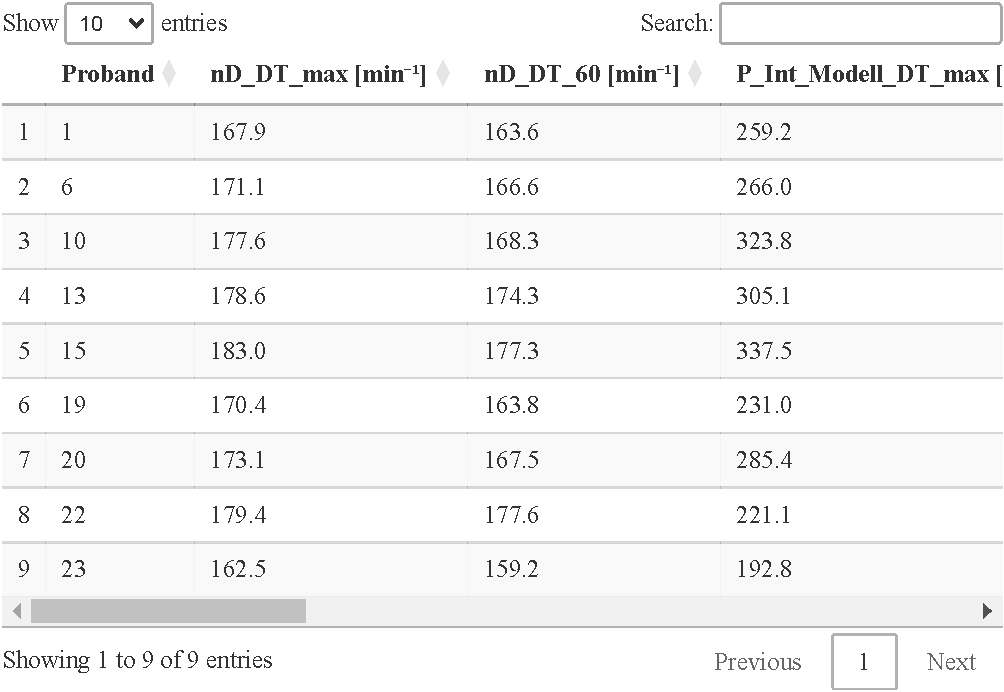
\includegraphics{Drehzahl_Stufentests_files/figure-pdf/tbl-DT_table-1.pdf}

}

\end{table}%

\end{tcolorbox}

\subsection{Physiologische Parameter des
Drehzahltests}\label{physiologische-parameter-des-drehzahltests}

Die folgenden Abbildungen zeigen die gemittelten Belastungsparameter
aller Probanden die individuellen Verläufe der Herzrate, der
respiratorischen Parameter \(\dot{V}O_{2}\) und \(\dot{V}CO_{2}\) sowie
der mechanischen Leistung P\textsubscript{mech} über die Zeit für die
Stufentests im Sitzen und Stehen.

\subsection{MW}

\begin{figure}

\centering{

\includegraphics[width=11.45833in,height=4.6875in]{images/p_DT_gemittelt.html}

}

\caption{\label{fig-DT_gemittelt}Gemittelte Belastungsparameter aller
Drehzaltests}

\end{figure}%

\subsection{Proband 01}

\begin{figure}

\centering{

\includegraphics[width=11.45833in,height=4.6875in]{images/p_Drehzahltest_1.html}

}

\caption{\label{fig-DT_1}Belastungsparameter während des Drehzahltests:
Proband 01}

\end{figure}%

\subsection{Proband 06}

\begin{figure}

\centering{

\includegraphics[width=11.45833in,height=4.6875in]{images/p_Drehzahltest_6.html}

}

\caption{\label{fig-DT_6}Belastungsparameter während des Drehzahltests:
Proband 06}

\end{figure}%

\subsection{Proband 10}

\begin{figure}

\centering{

\includegraphics[width=11.45833in,height=4.6875in]{images/p_Drehzahltest_10.html}

}

\caption{\label{fig-DT_10}Belastungsparameter während des Drehzahltests:
Proband 10}

\end{figure}%

\subsection{Proband 13}

\begin{figure}

\centering{

\includegraphics[width=11.45833in,height=4.6875in]{images/p_Drehzahltest_13.html}

}

\caption{\label{fig-DT_13}Belastungsparameter während des Drehzahltests:
Proband 13}

\end{figure}%

\subsection{Proband 15}

\begin{figure}

\centering{

\includegraphics[width=11.45833in,height=4.6875in]{images/p_Drehzahltest_15.html}

}

\caption{\label{fig-DT_15}Belastungsparameter während des Drehzahltests:
Proband 15}

\end{figure}%

\subsection{Proband 19}

\begin{figure}

\centering{

\includegraphics[width=11.45833in,height=4.6875in]{images/p_Drehzahltest_19.html}

}

\caption{\label{fig-DT_19}Belastungsparameter während des Drehzahltests:
Proband 19}

\end{figure}%

\subsection{Proband 20}

\begin{figure}

\centering{

\includegraphics[width=11.45833in,height=4.6875in]{images/p_Drehzahltest_20.html}

}

\caption{\label{fig-DT_20}Belastungsparameter während des Drehzahltests:
Proband 20}

\end{figure}%

\subsection{Proband 22}

\begin{figure}

\centering{

\includegraphics[width=11.45833in,height=4.6875in]{images/p_Drehzahltest_22.html}

}

\caption{\label{fig-DT_22}Belastungsparameter während des Drehzahltests:
Proband 22}

\end{figure}%

\subsection{Proband 23}

\begin{figure}

\centering{

\includegraphics[width=11.45833in,height=4.6875in]{images/p_Drehzahltest_23.html}

}

\caption{\label{fig-DT_23}Belastungsparameter während des Drehzahltests:
Proband 23}

\end{figure}%

\section{Quellenverzeichnis}\label{quellenverzeichnis}

\phantomsection\label{refs}
\begin{CSLReferences}{1}{0}
\bibitem[\citeproctext]{ref-Hagberg1981}
Hagberg, J. M., Mullin, J. P., Giese, M. D., \& Spitznagel, E. (1981).
{Effect of pedaling rate on submaximal exercise responses of competitive
cyclists}. \emph{Journal of Applied Physiology Respiratory Environmental
and Exercise Physiology}, \emph{51}(2), 447--451.
\url{https://doi.org/10.1152/jappl.1981.51.2.447}

\bibitem[\citeproctext]{ref-Heck2022}
Heck, H., Bartmus, U., \& Grabow, V. (2022). \emph{{Laktat}} (1. Aufl.,
S. 662). Springer Berlin Heidelberg.

\bibitem[\citeproctext]{ref-Hintzy-Cloutier2003}
Hintzy-Cloutier, F., Zameziati, K., \& Belli, A. (2003).
\href{https://www.ncbi.nlm.nih.gov/pubmed/12629462}{{Influence of the
base-line determination on work efficiency during submaximal cycling}}.
\emph{Journal of Sports Medicine and Physical Fitness}, \emph{43}(1),
51--56.

\bibitem[\citeproctext]{ref-Oezyener2001}
Özyener, F., Rossiter, H. B., Ward, S. A., \& Whipp, B. J. (2001).
{Influence of exercise intensity on the on- and off-transient kinetics
of pulmonary oxygen uptake in humans.} \emph{The Journal of physiology},
\emph{533}(Pt 3), 891--902.
\url{https://doi.org/10.1111/j.1469-7793.2001.t01-1-00891.x}

\bibitem[\citeproctext]{ref-Rassouli2015}
Rassouli, F., \& Thurnheer, R. (2015). {Spiroergometrie -- Indikation,
Durchf{ü}hrung und Interpretation}. \emph{Swiss Medical Forum ‒
Schweizerisches Medizin-Forum}, \emph{15}(1415), 315--321.
\url{https://doi.org/10.4414/smf.2015.02227}

\bibitem[\citeproctext]{ref-Wasserman2011}
Wasserman, K., Hansen, J. E., Sue, D. Y., Stringer, W. W., Sietsema, K.
E., Sun, X. G., \& Whipp, B. J. (2011). \emph{{Principles of exercise
testing and interpretation: Including pathophysiology and clinical
applications: Fifth edition}} (S. 1--592).
\url{https://doi.org/10.1097/00024382-200014010-00017}

\end{CSLReferences}



\end{document}
